%! Author = alison o'connor
%! Date = 19/10/22
%! Results from PAPERA/BO/RESULTS/V1
%%
%% Copyright 2007-2019 Elsevier Ltd
%%
%% This file is part of the 'Elsarticle Bundle'.
%% ---------------------------------------------
%%
%% It may be distributed under the conditions of the LaTeX Project Public
%% License, either version 1.2 of this license or (at your option) any
%% later version. The latest version of this license is in
%%	http://www.latex-project.org/lppl.txt
%% and version 1.2 or later is part of all distributions of LaTeX
%% version 1999/12/01 or later.
%%
%% The list of all files belonging to the 'Elsarticle Bundle' is
%% given in the file `manifest.txt'.
%%
%% Template article for Elsevier's document class `elsarticle'
%% with harvard style bibliographic references

\documentclass[preprint, review, 12pt]{elsarticle}

%% Use the option review to obtain double line spacing
%% \documentclass[preprint,review,12pt]{elsarticle}

%% The amssymb package provides various useful mathematical symbols
\usepackage{amssymb}
%% The amsthm package provides extended theorem environments
%% \usepackage{amsthm}

%% The lineno packages adds line numbers. Start line numbering with
%% \begin{linenumbers}, end it with \end{linenumbers}. Or switch it on
%% for the whole article with \linenumbers.
%\usepackage{lineno}
%\linenumbers


%% MY PACKAGES
\usepackage{afterpage}
\usepackage{amsmath}
\usepackage{amsfonts}
\usepackage{amssymb}
\usepackage{array}
\usepackage{adjustbox}
\usepackage[bookmarks=false, breaklinks]{hyperref}
\hypersetup{colorlinks,
	linkcolor=blue,
	citecolor=blue,
	urlcolor=blue}
\usepackage{bm}
\usepackage{booktabs}
\usepackage{caption}
\usepackage{float}
\usepackage{gensymb}
\usepackage{wasysym}
\usepackage{import}
\usepackage[utf8]{inputenc}
\usepackage{tabularx}
\usepackage{multicol}
\usepackage{multirow}
\usepackage{siunitx}
\usepackage{subcaption}
\usepackage{placeins}
\usepackage{pdflscape}
\usepackage{longtable}
\usepackage[markup=underlined]{changes}
\newcolumntype{P}[1]{>{\centering\arraybackslash}p{#1}}
\usepackage{graphicx}
\graphicspath{{../../RESULTS/}{../FIGURES/}}
\renewcommand{\floatpagefraction}{.8}%
%%COLUMN WIDTHS FOR TABLES
\newcolumntype{b}{X}
\newcolumntype{s}{>{\hsize=.2\hsize}X}
\newcolumntype{m}{>{\hsize=.5\hsize}X}
\usepackage{soul}
%%%FORMATTING
\widowpenalty10000
\clubpenalty10000

\journal{European Journal of Mechanics A/Solids}


\begin{document}
	\begin{frontmatter}


		\title{A Machine Learning Approach to Automate Ductile Damage Parameter Selection using Finite Element Simulations}

		\author[1,2]{A.N. O'Connor\corref{cor1}}
		\ead{alison.oconnor@ul.ie}
		\author[1,3]{P.G. Mongan}
		\author[1,2,3]{N.P. O'Dowd}

		\address[1]{School of Engineering, University of Limerick, Ireland}
		\address[2]{Bernal Institute, University of Limerick, Ireland}
		\address[3]{Confirm Smart Manufacturing Research Centre, Ireland}

		\begin{abstract}

			Here Bayesian optimisation, a machine learning technique, in conjunction with finite element analysis is shown to successfully identify material model parameters in a ductile damage model.
			The Bayesian derived material model parameters result in simulated output with less than 2\% error compared to experimental data.
			The framework detailed here is fully autonomous, requiring data that can be derived from a simple tensile test.
			This framework has been successfully deployed to three datasets of P91 material tested at ambient ($20~\degree$C) and higher ($500~\degree$C) temperatures.
		\end{abstract}

		\begin{highlights}
			%%% MAX 85 CHARACTERS INCLUDING SPACES
			\item Ductile damage model parameters are obtained from Bayesian optimisation and FE.
			\item Errors of less than 2\%, comparing experimental and simulation data, are reported.
			\item The automated approach requires minimal user input.
%			\item Material parameters in a ductile damage model have been obtained using a combination of Bayesian optimisation and finite element analysis.
%			\item The automated approach can be used to analyse materials data with limited user interaction providing a potential for systematic study of large material data sets.
		\end{highlights}

		\begin{keyword}
			machine learning;
			Bayesian optimisation;
			ductile damage;
			parameter selection;
		\end{keyword}

	\end{frontmatter}

	%%%%%%%%%%%%%%%%%%%%%%%%%%%
	\section{Introduction}
	\label{h:introduction}

	The tensile test is a standard test method~\cite{ENISO6892} that provides information about the mechanical properties of metallic materials.
	In cases where experimental data are limited finite element (FE) simulations can be used to simulate the mechanical behaviour of materials and examine hypotheses that cannot be experimentally investigated.
	The FE method offers a level of detail not obtainable from analytical solutions but is relatively computationally expensive and ultimately relies on experimental data for validation.
	Ductile damage modelling can be used in conjunction with FE simulations to represent mechanical behaviour of metals under high strain conditions when damage mechanisms are important~\cite{ABBASSI2013, CHAHBOUB2019, ZHANG2021}.
	Such models are generally complex and require calibration parameters that are difficult to derive experimentally or analytically.
	Calibrating a ductile damage modelling can be considered a form of black box optimisation, where the inputs (calibration parameters) and outputs (data in a tensile test) are known but the functional relationship between the calibration parameters and the material mechanical response is unknown.
	Such an optimisation problem can be solved using machine learning, a term used to describe algorithms and/or statistical models that allow computers to select the best method of progression in a problem, without human interaction or explicit programming~\cite{BIKMKHAMETOV2020}.
	In particular, Bayesian optimisation (BO) has been shown to outperform other machine learning algorithms in solving black box optimisation problems~\cite{SNOEK2012}.
	Machine learning algorithms, informed directly by experimental and/or simulation data, have been successfully employed to solve numerous engineering problems across a wide range of applications~\cite{MONGAN2022, LIU2020, HEGDE2020}.
	BO is commonly used in machine learning for artificial neural network (ANN) hyperparameter selection~\cite{DEWANCKER2016, MONGAN2022, BIKMKHAMETOV2020, GHAVAMIAN2021} and has recently been used to identify material parameters in a viscoplastic material model~\cite{RYAN2022}.
	The versatility of BO makes it an attractive method for solving a wide variety of engineering challenges such as: material design ~\cite{ZHANG2020, CHUAQUI2021}, cardiac mechanics~\cite{BOROWSKA2022}, light emission for thin films~\cite{WANKERL2022} and manufacturing process improvements~\cite{MONGAN2022, GUNN2022}.
	In~\cite{ABENDROTH2006, ABBASSI2013, CHAHBOUB2019, CHEN2021} ANNs have been used to assess damage model parameters.
	However, ANNs require a significant number of FE simulations to `train' the model to recognise correlations and relationships between input values and results which is computationally expensive.
	This work demonstrates how BO can be used to automatically identify the material damage model parameters that best match experimental data from a tensile test, reducing the time associated with deriving parameter values and requiring minimal user intervention.
	A similar approach to that used in~\citet{RYAN2022} has been adopted, but in this case the approach is applied to ductile damage, using a Gurson model, rather than the rate sensitive viscoplasticity constitutive models examined in~\citet{RYAN2022}.

	\section{Material behaviour in FE simulations}
	\label{h:general_material_behaviour}

	A tensile test consists of a standardised specimen geometry that is loaded in one direction until complete separation of the specimen.
	Data are typically expressed in terms of engineering stress and strain ($\sigma_{eng}$ and $\epsilon_{eng}$, respectively), where stress and strain are derived from test measurements of test machine load and specimen displacement, respectively.
	For metals the relationship between stress and strain typically comprises three regions (see Figure~\ref{fig:eng_ss}): a linear region, a strain hardening region where stress increases non-linearly with strain, and a material damage region where stress decreases non-linearly with increasing strain.
	Several key mechanical properties derived from a tensile test are illustrated in Figure~\ref{fig:eng_ss}.
	The yield strength ($\sigma_y$) defines the stress at which material behaviour becomes non-linear.
	The linear region comprises data preceding the yield point of the material and the material stiffness or Young's modulus ($E$) is the slope of the stress-strain curve, as shown in Figure~\ref{fig:eng_ss}.
	Beyond $\sigma_y$ the slope of the stress-strain decreases and a local geometrical discontinuity known as a `neck' forms in the tensile specimen.
	The ultimate tensile strength, $\sigma_{UTS}$, denotes the maximum stress reached in the tensile test; beyond which the specimen's load bearing capacity degrades.
	The strain hardening region occurs for $\sigma_y \leq \sigma \leq \sigma_{UTS}$, as illustrated in Figure~\ref{fig:eng_ss}, and depicts a non-linear stress-strain relationship.
	\begin{figure}[!htbp]
		\centering
		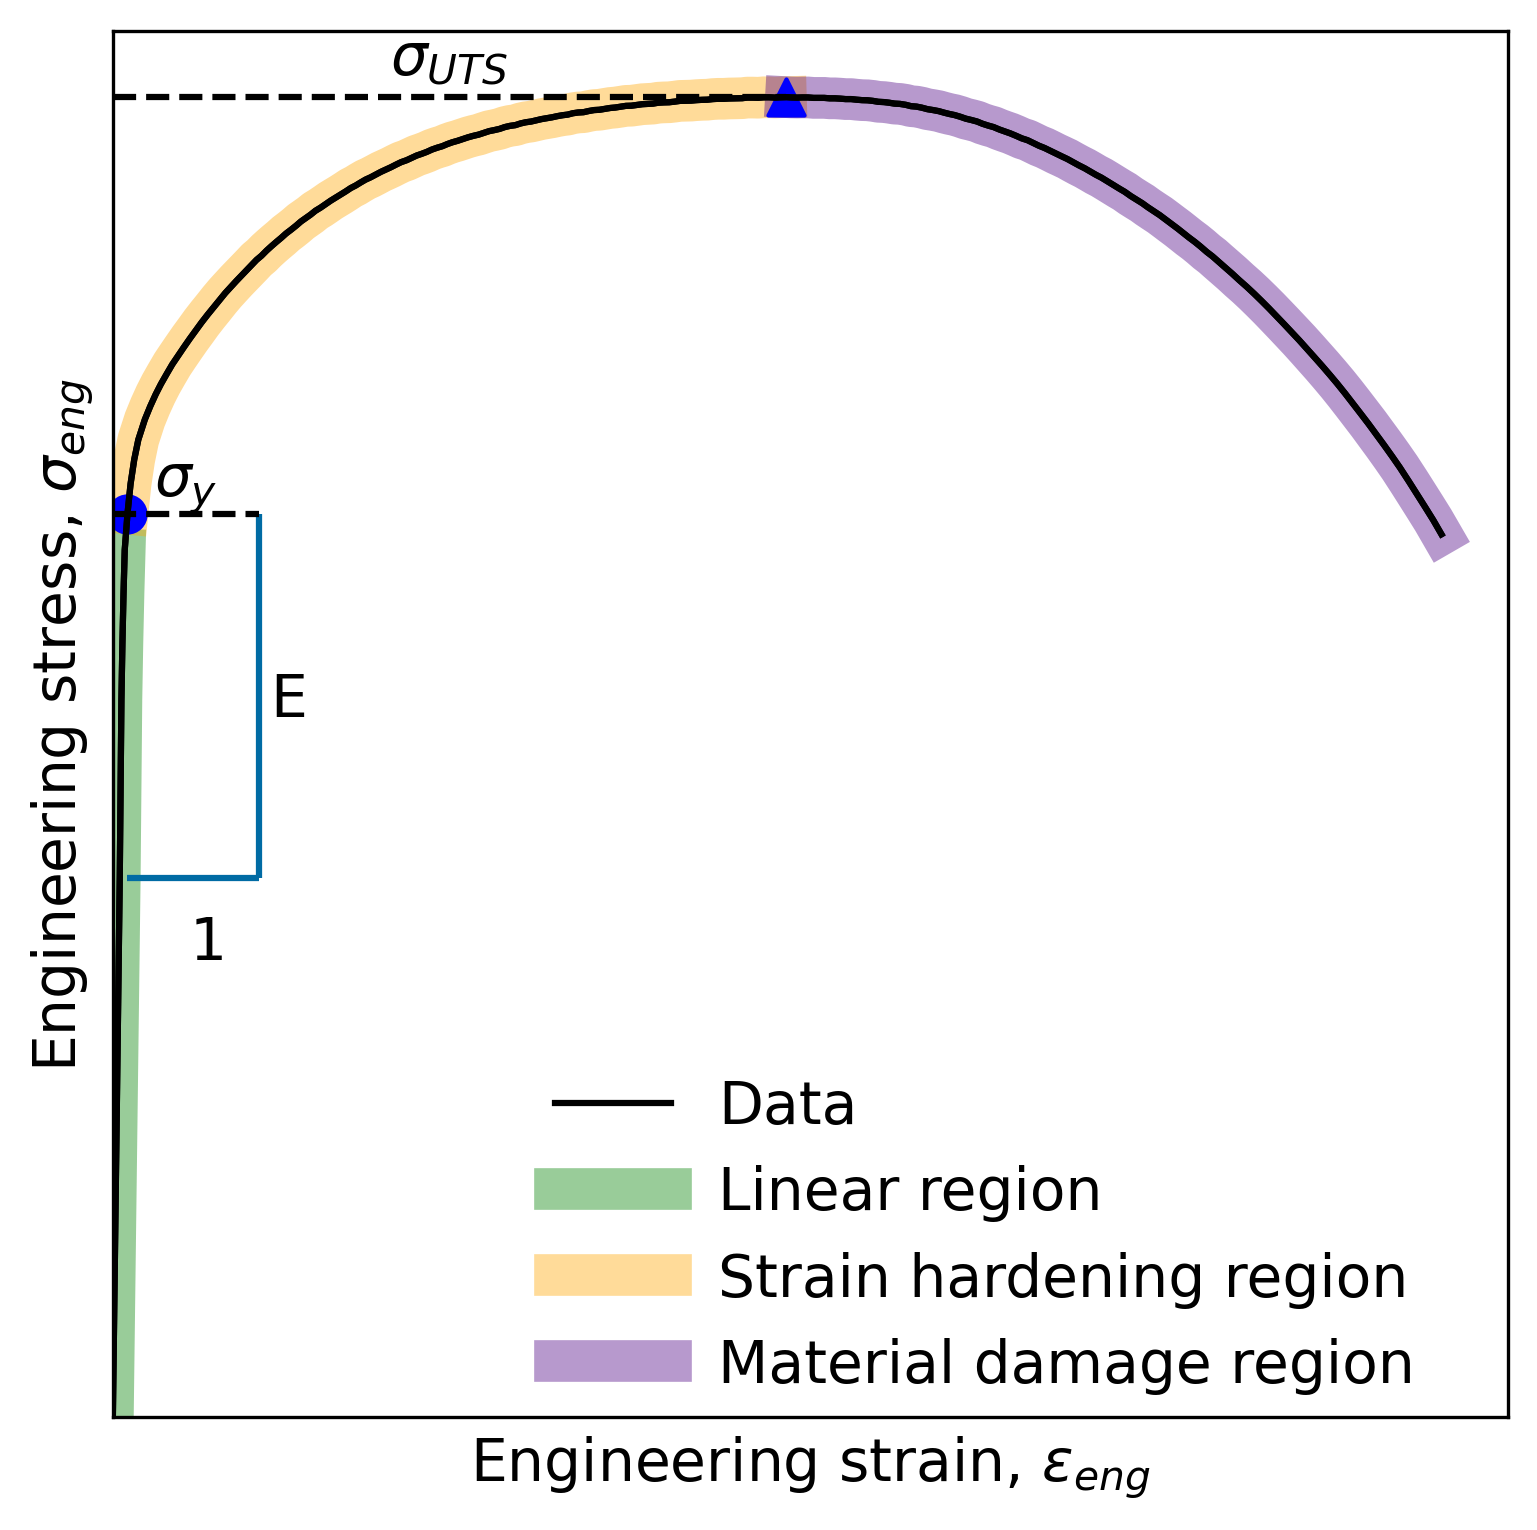
\includegraphics[width=\linewidth, height=0.4\textheight, keepaspectratio]{DIAGRAM_ENG_SS}
		\caption{Illustration depicting material behaviour during tensile test experiment.}
		\label{fig:eng_ss}
	\end{figure}
	The conversion from a load-displacement curve to an engineering stress-strain curve (Equations~\ref{eq:eng_stress}~and~\ref{eq:eng_strain}) used in Figure~\ref{fig:eng_ss}, assumes that the specimen geometry does not change during the test.
		\begin{equation}
		\sigma_{eng} = \frac{P}{A}
		\label{eq:eng_stress}
	\end{equation}

	\begin{equation}
		\varepsilon_{eng} = \frac{\Delta l}{l_o}
		\label{eq:eng_strain}
	\end{equation}
	Where $P$ represents the force applied to the specimen, $A$ the specimen cross-sectional area, $\Delta l$ the change in length of the specimen and $l_0$ the original length.
	However, the cross-section area of the specimen decreases continuously with increasing load, due to the Poisson effect ~\cite{YOUNG2001}.
	To account for this geometric change so-called true stress and true strain ($\sigma_{true}$ and $\epsilon_{true}$, respectively) are defined in Equations~\ref{eq:eng_stress}~and~\ref{eq:true_strain}.

	\begin{equation}
		\sigma_{true} = \sigma_{eng} \left( 1 + \varepsilon_{eng} \right)
		\label{eq:true_stress}
	\end{equation}

	\begin{equation}
		\varepsilon_{true} = ln\left( 1 + \varepsilon_{eng} \right)
		\label{eq:true_strain}
	\end{equation}

	This equation becomes increasingly inaccurate as the neck develops due to the non-uniformity of stress and strain in the neck.
	Therefore, in this work for $\sigma > \sigma_{UTS}$, the true stress is interpolated from the values for $\sigma \leq \sigma_{UTS}$, with the understanding that, in the absence of damage, the true stress always increases with increasing strain.
	Here, a linear relationship between true stress and true strain, with slope $m$, for $\sigma \ge \sigma_{UTS}$ is assumed.
	The parameter $m$ is unknown and is calibrated as part of the BO, as discussed later.

	\subsection{The damage model}
	\label{h:damage_model}

	A popular damage model, used to describe the softening behaviour seen in the material damage region of Figure~\ref{fig:eng_ss}, is the Gurson-Tvergaard-Needleman (GTN) model~\cite{WCISLIK2016, CHAHBOUB2019, TVERGAARD1984a}.
	The parameters are typically estimated by conducting numerical simulations, manually iterating the relevant parameter value, and matching the simulation result to experimental data.

	The GTN model response for a tensile test is described in Equation~\ref{eq:gtn_yield}, where $\sigma$ is the current (uniaxial) stress, $\sigma_y$ is the material yield strength, $f$ is the current void volume fraction (the ratio of the volume of voids to the total material volume) and $q_1$, $q_2$, and $q_3$ are material parameters,
	\begin{equation}
		\left( \frac{\sigma}{\sigma_y} \right)^2 + 2q_{1}f\left( \cosh \frac{q_2 \sigma}{2\sigma_y} \right) - q_3 f^2 = 1.
		\label{eq:gtn_yield}
	\end{equation}

	The rate of change of the void volume fraction, $f$, is described by Equation~\ref{eq:vvf} where $\dot{f}_n$ and $\dot{f}_g$ represent the void nucleation rate and void growth rate, respectively,

	\begin{equation}
		\dot{f} = \dot{f}_n + \dot{f}_g.
		\label{eq:vvf}
	\end{equation}
	The void growth rate, $\dot{f}_g$, is obtained from conservation of mass,
	\begin{equation}
		\dot{f}_g = (1-f)\dot{\varepsilon},
		\label{eq:void_growth}
	\end{equation}
	while the void nucleation rate, $\dot{f}_n$, is given by Equation~\ref{eq:void_nucleation}, where $\varepsilon^p_m$ is the plastic strain of the unvoided (matrix) material, and $f_N$, $S_N$ and $\varepsilon_N$, are material parameters.

	\begin{equation}
		\dot{f}_n = \frac{f_N}{S_N \sqrt{2\pi}} \exp \left[ -\frac{1}{2} \left( \frac{{\varepsilon}_m^p -\varepsilon_N}{S_N} \right) ^ 2 \right] \dot{\varepsilon}_m^p
		\label{eq:void_nucleation}
	\end{equation}

	Since, the void volume, $f$, is defined through a rate equation, the initial void volume fraction, $f_0$, must also be defined.
	Hence, there are a total of seven parameters in the GTN ductile damage model to fit using BO: $q_1$, $q_2$, $q_3$, $S_N$, $f_N$, $\varepsilon_N$, and $f_0$.
	Including the slope of the true stress-true strain curve for $\sigma>\sigma_{UTS}$, $m$, gives a total of eight parameters.

	\section{The Bayesian Optimisation Framework}
	\label{h:general_bo}

	The goal of BO is to find the global minimum of an unknown (black box) function.
	There are two key ingredients to a BO framework: a surrogate model and a loss function.
	The surrogate model, sometimes called a probabilistic model, describes the BO's current knowledge about the unknown function based on observed data.
	The loss function describes how well the previously observed data are optimised (i.e.\ converging towards a global minimum)~\cite{SHAHRIARI2016}.
	The surrogate model and loss function work jointly with an acquisition function, which controls how the BO explores the parameter space.
	The surrogate model, $f(x)$, is determined using Gaussian process regression (GPR) on inputs, $x$, the observed data related to the unknown function.
	A Gaussian process is a collection of random variables, many of which have consistent, joint Gaussian distributions, specified by the covariance function~\cite{RASMUSSEN2004, RASMUSSEN2006} (see Section~\ref{h:covariance_function} for further details on the covariance function).

	The probability distribution generated by GPR is based on a ranking system, where input $x$ is evaluated as $f(x)$ and $f(x)$ is ranked in terms of its performance relative to the loss function.
	In this work the loss function is the mean average percentage error (MAPE) which quantifies the similarity between simulated and experimental data (see Section~\ref{h:mape_detailed} for further detail).
	To minimise the loss function the L-BFGS-B optimisation algorithm~\cite{ZHU1997} is used.
	This algorithm uses historical gradient evaluations of $f(x)$ to construct an approximation of the unknown function.

	In order to set reasonable bounds to the possible solutions of the problem, a parameter space is defined, within which the BO algorithm searches for values.
	The parameter space of the current problem is defined in Table~\ref{tab:parameter_space_all} for the GTN parameters, based on information in the literature for similar materials~\cite{KIRAN2014,MEADE2020,DASSAULT2021}.
	The process used to define the bounds for $m$ is outlined in detail in Section~\ref{h:tensile_tests}.

	\begin{table}[!htbp]
\centering
\caption{Parameter space representing the minimum and maximum boundary for each parameter}
\label{tab:parameter_space_all}
\begin{tabular}{lccc}
\toprule
\textbf{Dataset} &  \textbf{Parameter} & \textbf{Minimum} & \textbf{Maximum}\\
\midrule
%{1-3} &    \textbf{$q_1$} &  0.90 &    1.60 \\
%{1-3} &    \textbf{$q_2$} &  0.90 &    1.10 \\
%{1-3} &    \textbf{$q_3$} &  0.81 &    2.56 \\
%{1-3} &    \textbf{$\epsilon_N$} &  0.25 &    0.40\\
%{1-3} &    \textbf{$f_N$} &  0.03 &    0.09 \\
%{1-3} &    \textbf{$s_N$} &  0.10 &    0.20 \\
%{1-3} &    \textbf{$f_0$} &  1.3\times 10^{-3} &    1.5\times 10^{-3} \\
%{1} &    \textbf{$m$} &  0 &  800 \\
%{2} &    \textbf{$m$} &  0 &  1100 \\
%{3} &    \textbf{$m$} &  0 &  800 \\
%% 3 SIGNIFICANT FIGURES
{1-3} &    \textbf{$q_1$} &  9.00\times 10^{-1} &    1.60 \\
{1-3} &    \textbf{$q_2$} &  9.00\times 10^{-1} &    1.10 \\
{1-3} &    \textbf{$q_3$} &  8.10\times 10^{-1} &    2.56 \\
{1-3} &    \textbf{$\epsilon_N$} &  2.50\times 10^{-1} &    4.00\times 10^{-1}\\
{1-3} &    \textbf{$f_N$} &  3.00\times 10^{-1} &    9.00\times 10^{-2} \\
{1-3} &    \textbf{$s_N$} &  1.00\times 10^{-1} &    2.00\times 10^{-1} \\
{1-3} &    \textbf{$f_0$} &  1.30\times 10^{-3} &    1.50\times 10^{-3} \\
{1} &    \textbf{$m$} &  0 &  800 \\
{2} &    \textbf{$m$} &  0 &  1100 \\
{3} &    \textbf{$m$} &  0 &  800 \\
\bottomrule
\end{tabular}
\end{table}

 	%%%%%%%%%%%%%%%%%%%%%%%%%%%
	\subsection{The covariance function}
	\label{h:covariance_function}

	The covariance function used in the GPR has significant influence on the shape and characteristics of the surrogate function~\cite{MONGAN2022}.
	In this work a covariance function, $k(x_i, x_j)$, which uses a combination of the Mat\'ern, Constant and White noise (White) functions, as shown in Equation~\ref{eq:mykernel},
	\begin{equation}
		k(x_i, x_j) = \text{Mat\'ern} + \text{Constant} \times \text{White},
		\label{eq:mykernel}
	\end{equation}
	is implemented.
	As the shape and/or characteristics of the black box function are unknown this covariance kernel is designed to account for shifts in mean position (Constant), noise (White) and to model potentially multiple minima positions (Mat\'ern).
	The Mat\'ern covariance function is defined in Equation~\ref{eq:matern}~\cite{PEDREGOSA2011},
	\begin{equation}
		k(x_i, x_j) = \frac{1}{\Gamma \left( \nu \right)2^{\nu-1}} \left( \frac{\sqrt{2\nu}}{l} d\left( x_i, x_j \right) \right)^{\nu}K_{\nu} \left( \frac{\sqrt{2\nu}}{l} d\left( x_i, x_j \right) \right),
		\label{eq:matern}
	\end{equation}
	where $x_i$ and $x_j$ are input points, $d$ is the Euclidean distance, $K_{\nu}$ is a modified Bessel function and $\Gamma$ is the gamma function.
	The Constant covariance function, is defined in Equation~\ref{eq:constant_kernal}~\cite{PEDREGOSA2011},
	\begin{equation}
		k\left( x_i, x_j \right) = C; \forall \; x_i, x_j,
		\label{eq:constant_kernal}
	\end{equation}
	where $C$ is a constant.
	The White covariance function is defined in Equation~\ref{eq:white},
	\begin{equation}
		k(x_i, x_j) = \sigma^2 \delta_{ij},
		\label{eq:white}
	\end{equation}
 	where $\sigma^2$ is constant and $\delta_{ij}$ the Kronecker delta function.
	In this work the following kernel hyperparameters are fixed: $\nu=1$, $l=1$, $C=1$, $\sigma^2=1$.

	%%%%%%%%%%%%%%%%%
	\subsection{The loss function (MAPE)}
	\label{h:mape_detailed}

	The aim of this work is to minimise the difference between experimental test data and simulation outputs generated from a finite element (FE) analysis of the problem.
	The experimental data are measures of applied load and specimen extension.
	In this work mean average percentage error (MAPE), Equation~\ref{eq:mape}, is used to measure the similarity between experimental data and simulated output,
 	\begin{equation}
	\text{MAPE} = \frac{100}{n} \sum_i^n \left| \frac{P_{exp}^i - P_{sim}^i}{P_{exp}^i} \right|.
	\label{eq:mape}
	\end{equation}

	Here $P^i_{exp}$ represents each experimental load data point, $P_{sim}^i$ is the corresponding simulation load and $n$ the number of data points.
	MAPE provides an average measure of error over the full dataset with all data points equally weighted.

	%%%%%%%%%%%%%%%%%%%%%%%%%%%
	\subsection{The acquisition function, $\alpha$}
	\label{h:acquisition_function}

	In this work the upper confidence bound (UCB) acquisition function is employed.
	The UCB, Equation~\ref{eq:ucb}, identifies the new parameters through a weighted sum of the surrogate function, where $\mu \left(x \right)$ is the mean, and $\sigma \left(x \right)$, the variance, respectively~\cite{SHAHRIARI2016, DEATH2021},


	\begin{equation}
	\alpha_{UCB} \left( x \right) = \mu \left( x \right) + B\: \sigma\left( x \right).
	\label{eq:ucb}
	\end{equation}

	Exploration and exploitation balance how the BO model searches the parameter space.
	When $B$ is large (e.g.\ $B>2$) the acquisition function operates in exploratory mode; reducing the weight switches the model to exploitation mode.
	In exploration mode the new assessment point differs significantly from the previous iteration; exploratory mode returns a new assessment point close to that tested previously.
	In our work we have taken $B=2.5$.

	In addition to the weight, $B$, the acquisition function has two further hyperparameters: the number of random samples, $N_R$, and the number of optimisation samples, $N_O$.
	$N_R$ controls the size of the array over which the range of possible inputs are distributed $-$ increasing $N_R$ increases the precision of the GPR, thus reducing uncertainty.
	$N_O$ defines how many evaluations of the acquisition function are conducted and controls the level of uncertainty in the acquisition function $-$ increasing $N_O$ makes the optimisation process more robust.

	\subsection{Initialising the BO framework}
	\label{h:framework}

	BO requires a database of initial evaluated data within the parameter space.
	We use a design of experiment (DoE) approach,~\cite{UY2009, FRALEY2020}, to provide the initial evaluated data.
	DoE maximises the statistical significance of results with a minimised number of experiments.
	Table~\ref{tab:L12} shows a DoE array for 12 initial finite element simulations based on the maximum and minimum parameter space values, where values of 1 and 2 in Table~\ref{tab:L12} represent the minimum and maximum parameter bounds, respectively.

	\begin{table}[tb]
\centering
\caption{Design of experiments array for 8 parameters with each parameter at 2 levels.}
\label{tab:L12}
\begin{tabular}{lrrrrrrrr}
\toprule
{} & $P_1$ & $P_2$ & $P_3$ & $P_4$ & $P_5$ & $P_6$ & $P_7$ & $P_8$ \\
\midrule
\textbf{1 } &     1 &     1 &     1 &     1 &     1 &     1 &     1 &     1 \\
\textbf{2 } &     1 &     1 &     1 &     1 &     1 &     2 &     2 &     2 \\
\textbf{3 } &     1 &     1 &     2 &     2 &     2 &     1 &     1 &     1 \\
\textbf{4 } &     1 &     2 &     1 &     2 &     2 &     1 &     2 &     2 \\
\textbf{5 } &     1 &     2 &     2 &     1 &     2 &     2 &     1 &     2 \\
\textbf{6 } &     1 &     2 &     2 &     2 &     1 &     2 &     2 &     1 \\
\textbf{7 } &     2 &     1 &     2 &     2 &     1 &     1 &     2 &     2 \\
\textbf{8 } &     2 &     1 &     2 &     1 &     2 &     2 &     2 &     1 \\
\textbf{9 } &     2 &     1 &     1 &     2 &     2 &     2 &     1 &     2 \\
\textbf{10} &     2 &     2 &     2 &     1 &     1 &     1 &     1 &     2 \\
\textbf{11} &     2 &     2 &     1 &     2 &     1 &     2 &     1 &     1 \\
\textbf{12} &     2 &     2 &     1 &     1 &     2 &     1 &     2 &     1 \\
\bottomrule
\end{tabular}
\end{table}


	Figure~\ref{fig:doe_flowchart} shows a flowchart describing the DoE procedure.
	As illustrated in Figure~\ref{fig:doe_flowchart}, the user first defines the parameter space (here shown in Table~\ref{tab:parameter_space_all}).
	A DoE array (Table~\ref{tab:L12}) is defined and the DoE array is modified so that the minimum and maximum values (i.e.\ 1 and 2) are replaced by the user-defined parameter values(see Table~\ref{tab:parameter_space_all}).
	A finite element simulation is conducted for each row of the DoE array ($i_{max}$) is the number of (virtual) experiments in the DoE array, here 12.
	Results from the simulation are processed (see Section~\ref{h:fem} for details) and MAPE is calculated (Section~\ref{h:mape_detailed}) by comparing the simulated output to experimental data.
	After each analysis, $i$, the parameter values and the associated error measurement are appended to a csv file.

	\begin{figure}[!htbp]
		\centering
		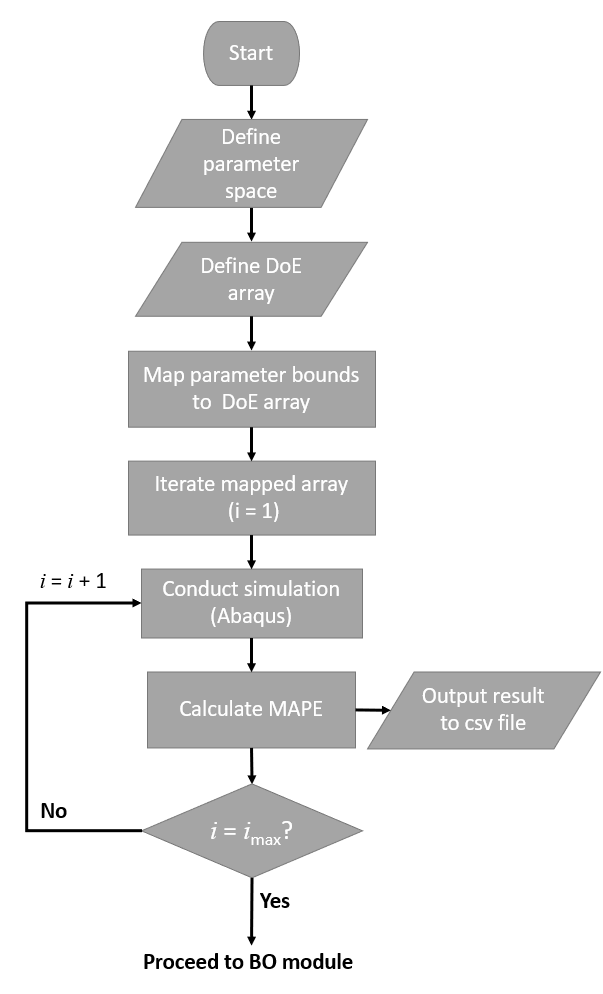
\includegraphics[width=\linewidth, height=0.8\textheight, keepaspectratio]{DOE_FLOWCHART}
		\caption{Flowchart demonstrating the design of experiments code procedure (prior to bayesian optimisation).}
		\label{fig:doe_flowchart}
	\end{figure}

	%%%%%%%%%%%%%%%%%
	\subsection{Implementation of the BO model}
	\label{h:bayesian_opt}
	The output of the DoE in Figure~\ref{fig:doe_flowchart} (a csv file of parameter values and error measurements) is used to initialise the Bayesian optimiser.
	Figure~\ref{fig:bo_flowchart} outlines the method: The DoE data are analysed by the GPR to create an initial surrogate model.
	GPR outputs are then provided to the acquisition function which identifies new parameter values based on ranking the DoE data.
	A new finite element simulation, using parameter values obtained from the acquisition function, is then conducted.
	Again simulation data is compared to the experiment and the MAPE is calculated.
	Acquisition function parameter values and error measurement data are appended to the existing csv file.
	The algorithm iterates until the MAPE is less than 2\% or a maximum number of iterations ($j_{max}$) is achieved.
	In the current approach, to ensure that BO is always carried out the analysis is not terminated if $\text{MAPE} < 2$\% in the DoE.

	\begin{figure}[!htbp]
		\centering
		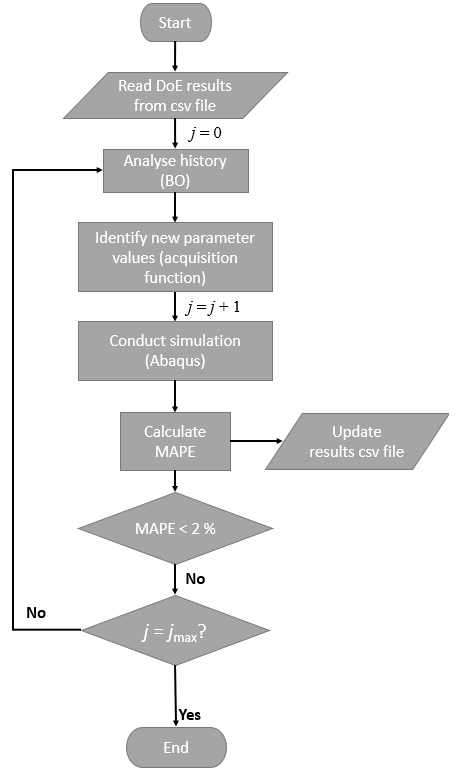
\includegraphics[width=\linewidth, height=0.8\textheight, keepaspectratio]{BO_FLOWCHART}
		\caption{Flowchart depicting code procedure for Bayesian optimisation.}
		\label{fig:bo_flowchart}
	\end{figure}

	%%%%%%%%%%%%%%%%%%%%%%%%%%%
	\section{Analysis of Experimental Data}
	\label{h:tensile_tests}

	Three experimental tensile test results are shown in Figure~\ref{fig:exp_test_results} for the material of interest (P91, a piping steel).
	Datasets 1 and 2 were conducted under identical test conditions, so Dataset 2 can be considered a repeat test.

	\begin{figure}[!htbp]
		\centering
		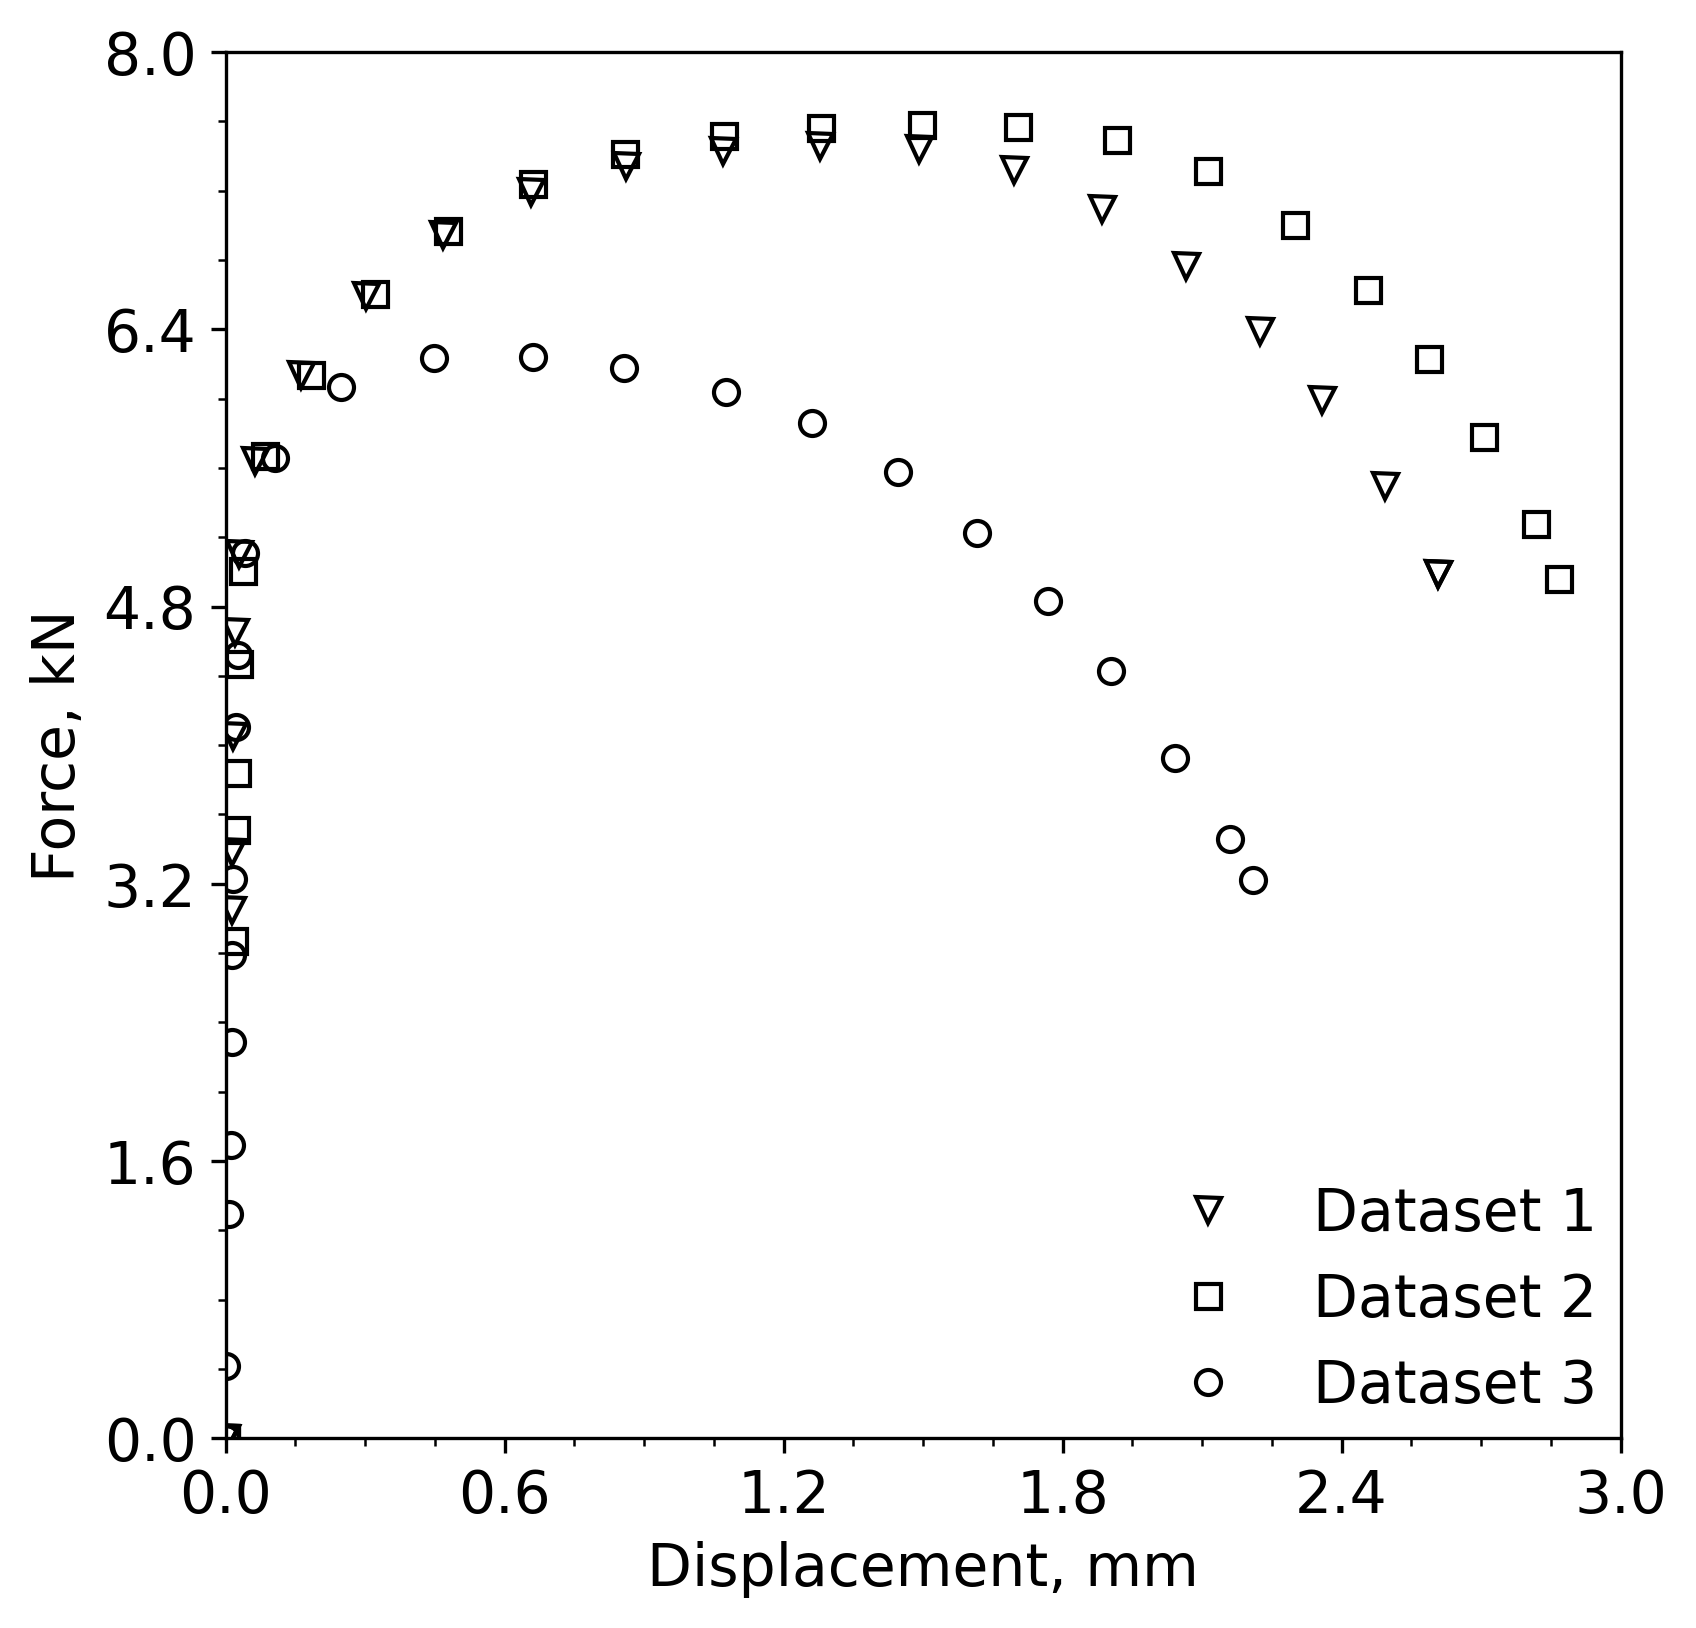
\includegraphics[width=\linewidth, height=0.4\textheight, keepaspectratio]{EXPERIMENTAL_RESULTS}
		\caption{Experimental tensile test results for P91 material at test temperatures of 20~\degree C (Datasets 1 and 2) and 500~\degree C (Dataset 3). Note: Markers are placed as specific intervals for data visibility purposes. Higher data acquistion rate was used during testing.}
		\label{fig:exp_test_results}
	\end{figure}

	%%%%%%%%%%%%%%%%%
	\subsection{Assessment of linear data}
	\label{h:linear_region}
	 As discussed in Section~\ref{h:general_material_behaviour}, two material parameters are required in the linear (elastic) region: Young's modulus, $E$, and yield strength, $\sigma_y$.
	As the choice of $\sigma_y$, influences the value of $E$, these are obtained by an iterative process (outside the BO framework).
	The region over which $\sigma_y$ is evaluated is solved iteratively and Young's modulus, $E$, is calculated by employing linear regression to fit all data below the selected yield strength.	Figure~\ref{fig:linear_region} shows the result of the assessment for each of the three datasets.

	\begin{figure}[!htbp]
		\centering
		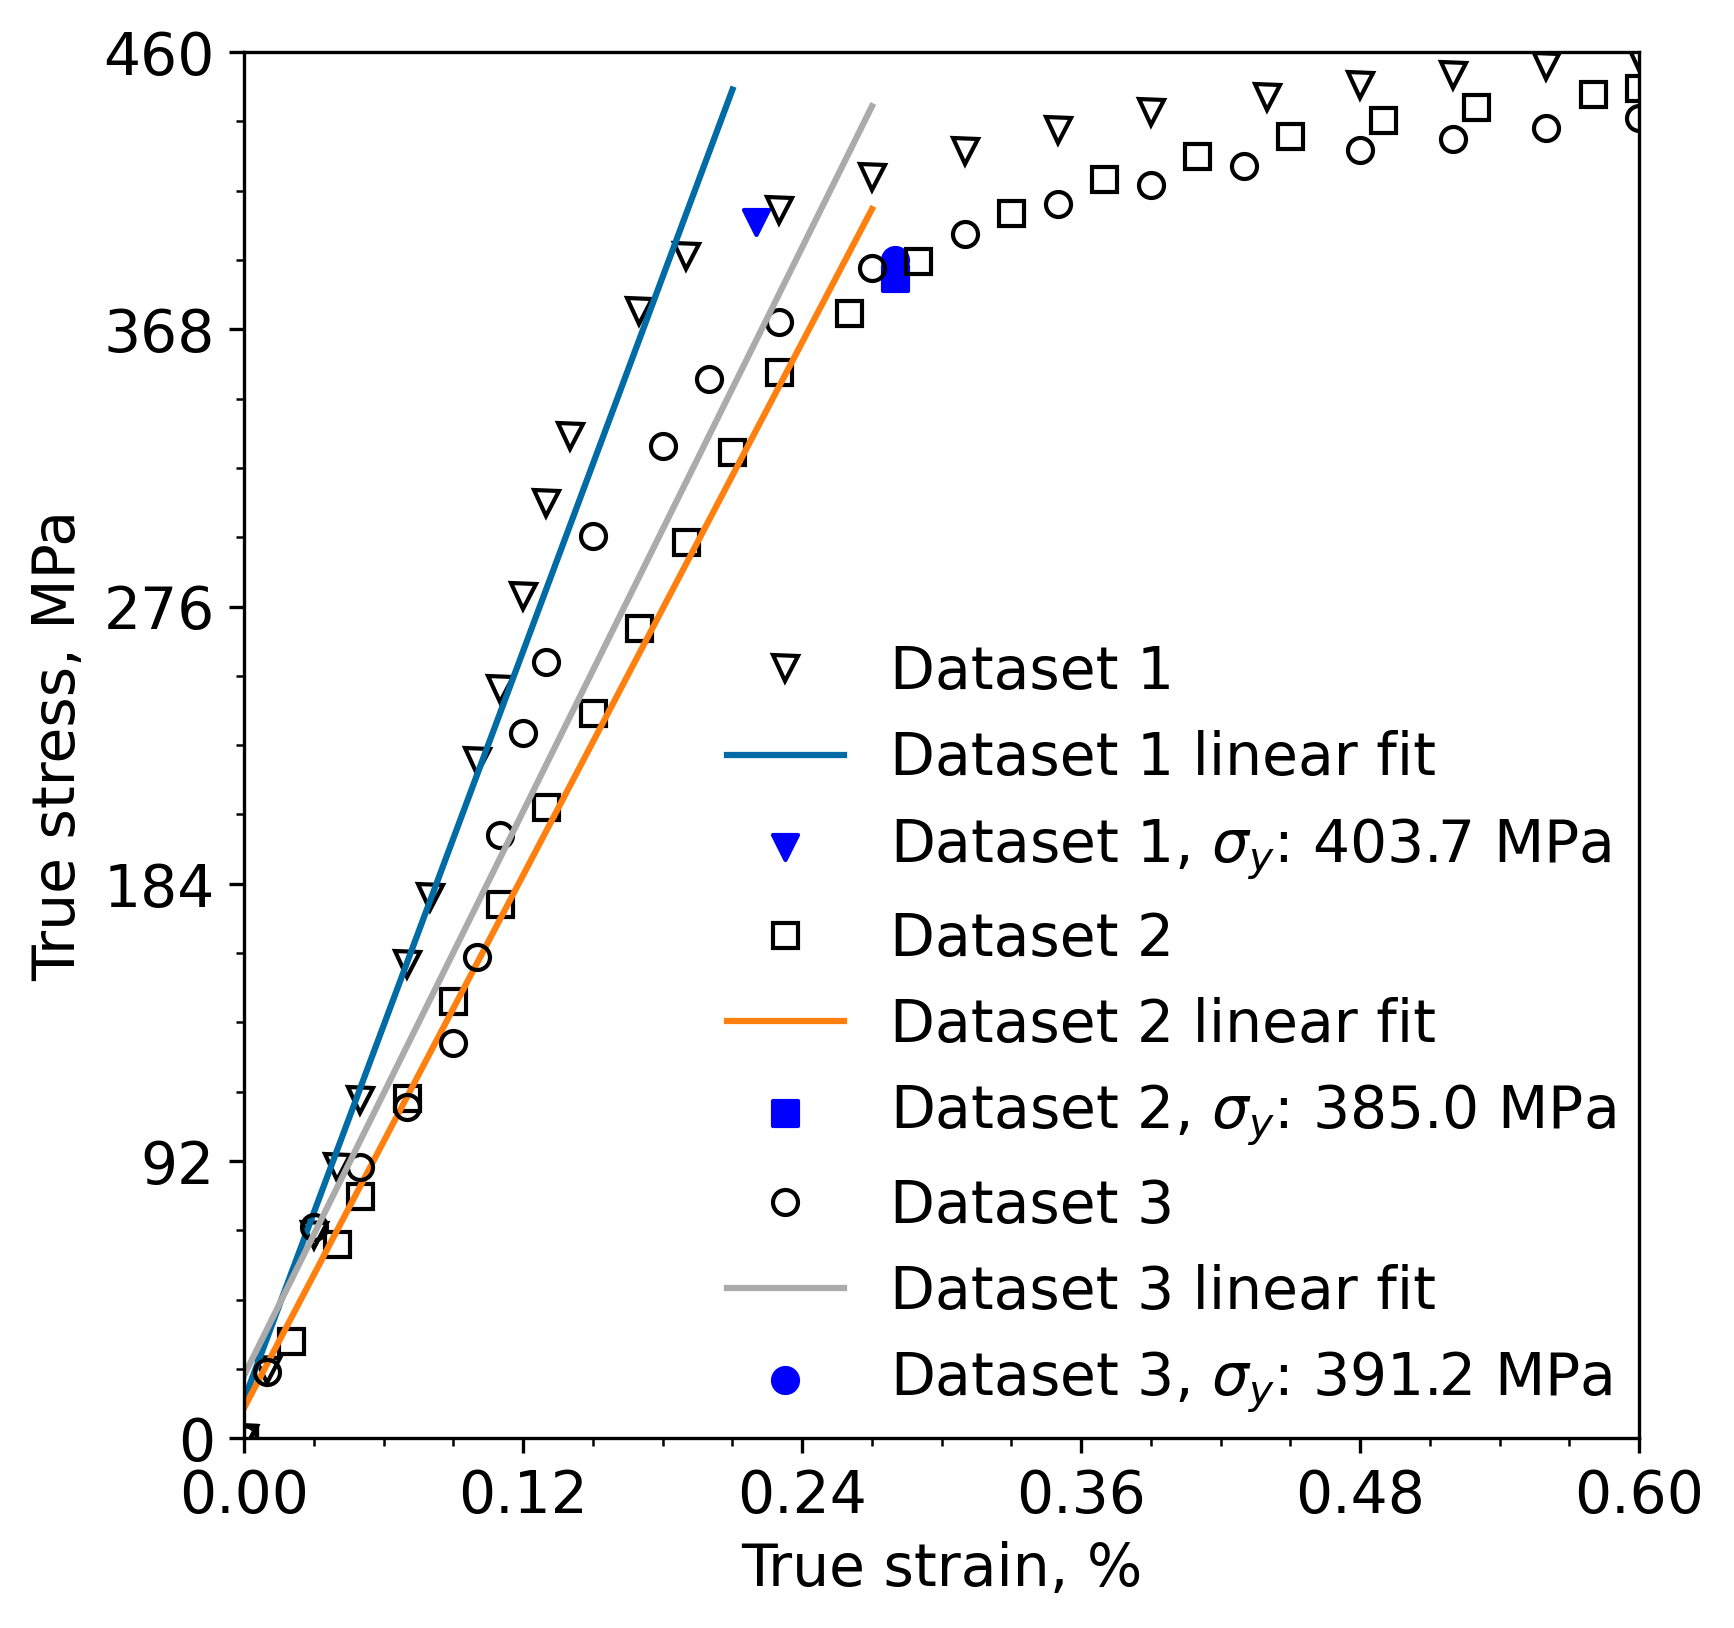
\includegraphics[width=\linewidth, height=0.4\textheight, keepaspectratio]{SECOND_DERIV}
		\caption{True stress - true strain relationship for three experimental tests.}
		\label{fig:linear_region}
	\end{figure}

	To extrapolate data beyond $\sigma_{UTS}$ we assume a linear relationship between true stress and plastic strain.
	The slope of the extrapolated line, parameter $m$, is one of the eight parameters determined by the BO framework.
	The range of $m$ is dependent on the material; the minimum value is 0 (as in Figure~\ref{fig:extending_uts}) and the maximum value is selected by considering all potential slopes from the data for $\sigma<\sigma_{UTS}$.
 	The true stress-true strain curve is then extrapolated linearly beyond $\sigma_{UTS}$ with a slope $m$, as shown in Figure~\ref{fig:extending_uts} for Dataset 1.

	\begin{figure}[!htbp]
		\centering
		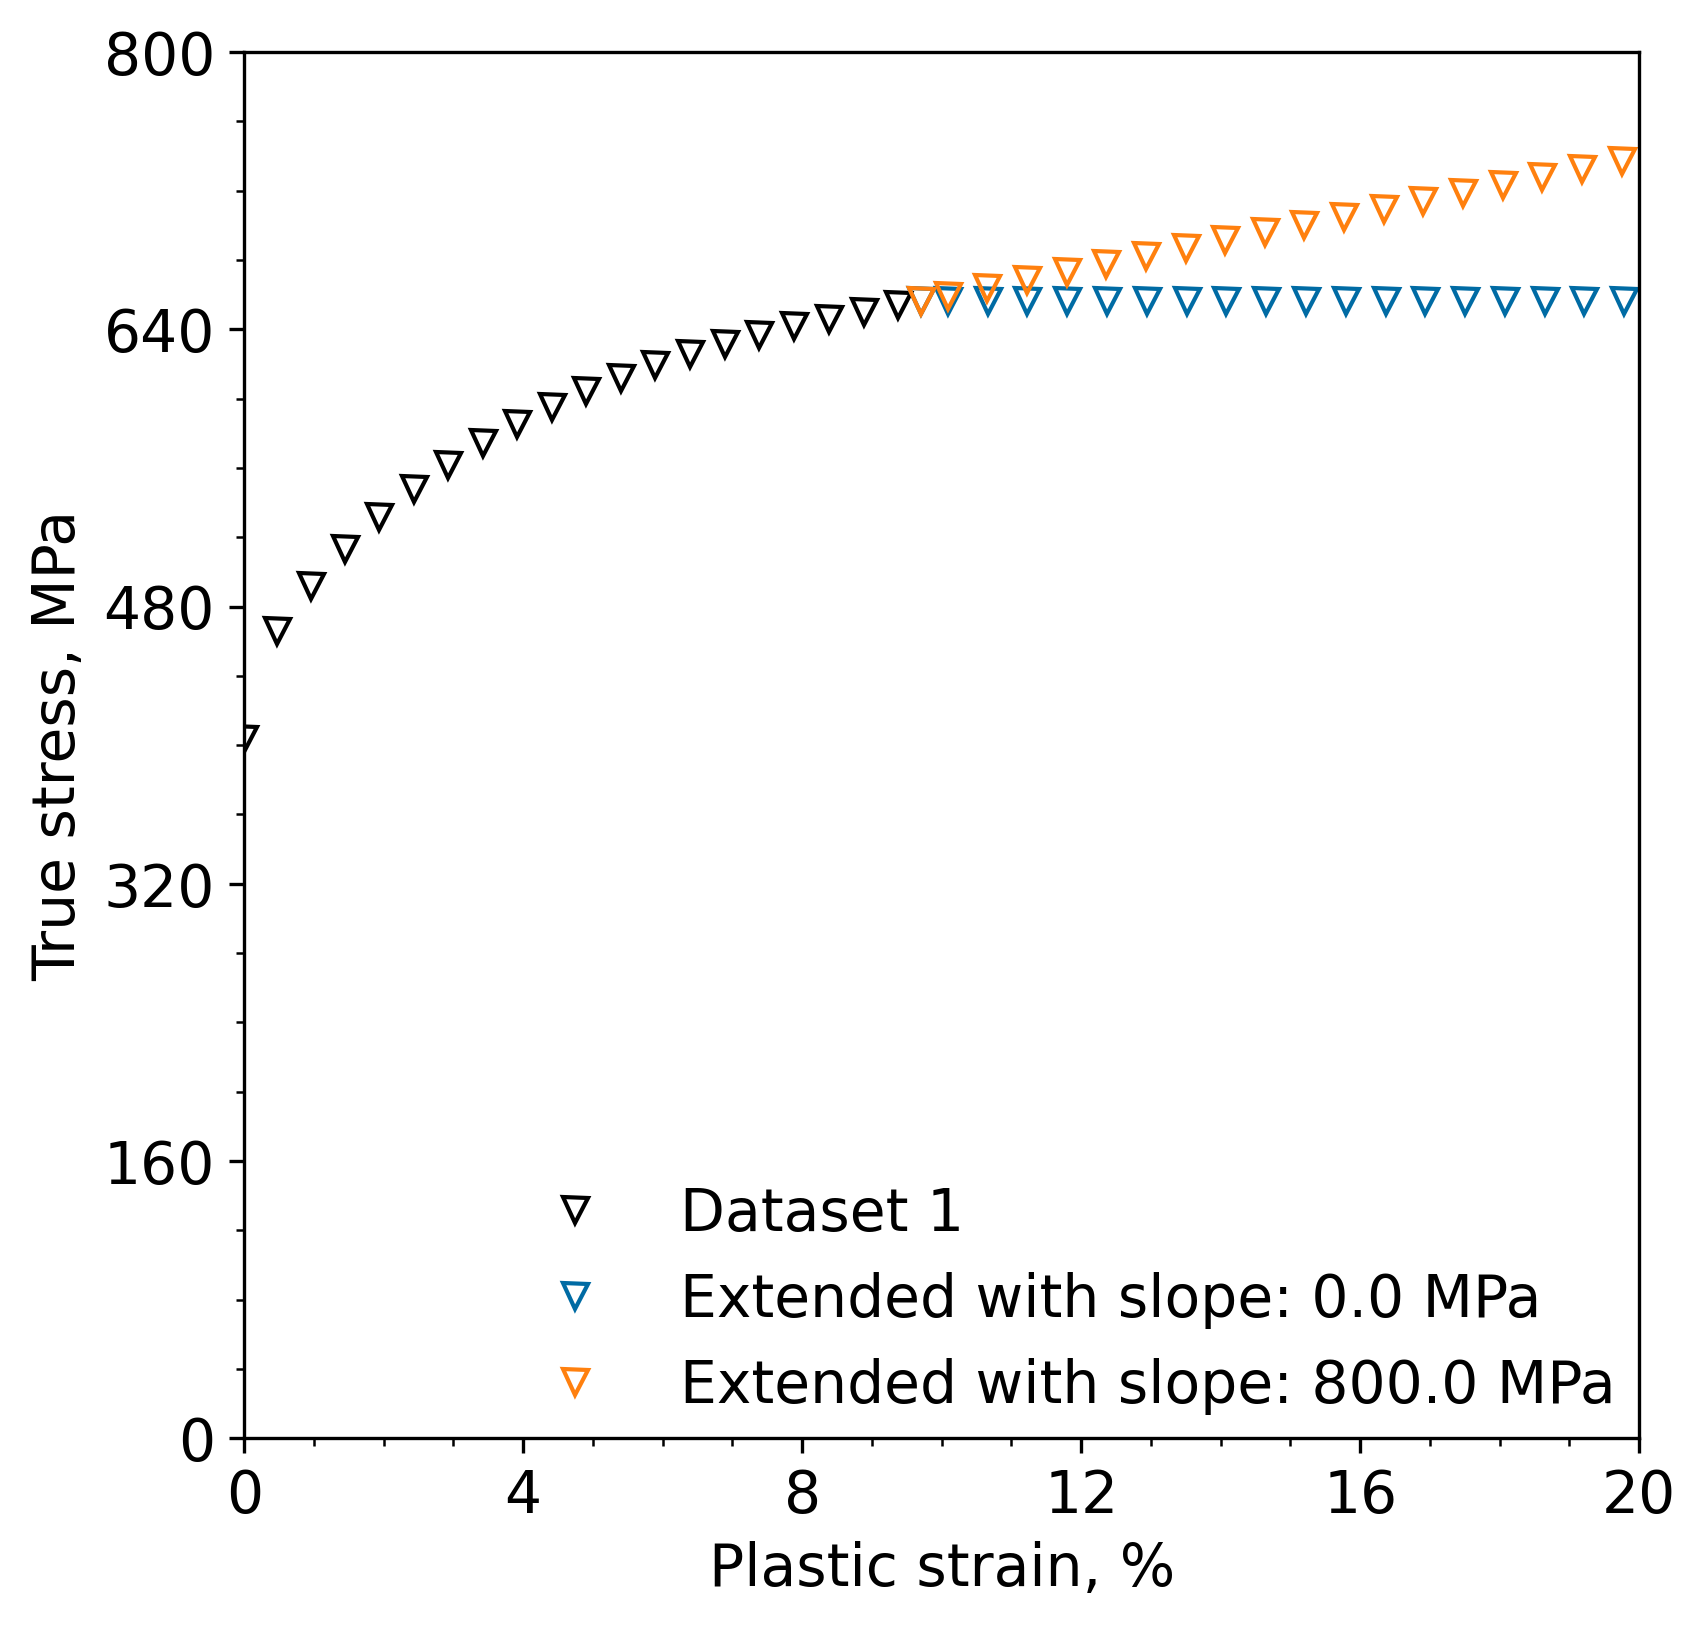
\includegraphics[width=\linewidth, height=0.4\textheight, keepaspectratio]{ABAQUS_SLOPE_COMPARISON}
		\caption{True stress - plastic strain relationship for dataset 1. Test data are shown using black markers. Two parameter values (minimum and maximum) are distingushed using coloured markers.}
		\label{fig:extending_uts}
	\end{figure}

	%%%%%%%%%%%%%%%%%%%%%%%%%%%
	\section{FE Modelling of Tensile Tests}
	\label{h:fem}

	Finite element modelling was conducted using Abaqus/Explicit~\cite{DASSAULT2021} (Explicit).
	Explicit uses a dynamic solver, and here a mass scaling factor of 10 is used to reduce computation time~\cite{DASSAULT2021}.
	The model was meshed using 4664 linear, reduced integration axisymmetric (CAX4R) elements.
	The smallest element size is 0.09~mm.

	The experimental tensile test geometry is shown in Figure~\ref{fig:fe_model}.
	The use of a 2D axisymmetric model reduces the computational expense of the simulation.
	Following the approach in~\cite{DASSAULT2021} for modelling of necking, a small imperfection is introduced at the bottom right hand corner of the model, as shown in Figure~\ref{fig:fe_model}, to provide a site for specimen necking at large displacements.

	\begin{figure}[!htbp]
		\centering
		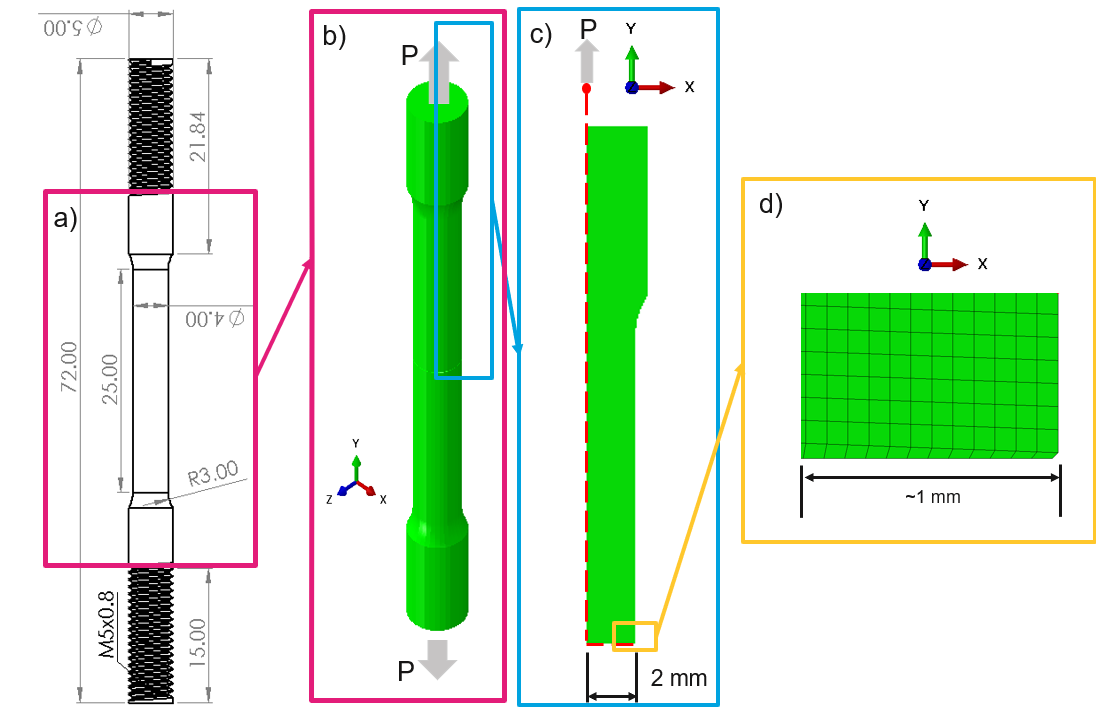
\includegraphics[width=\linewidth, height=0.5\textheight, keepaspectratio]{MODEL_3D_2D}
		\caption{ (a) Tensile specimen (all dimensions in mm) (b) 3D visualisation of the test specimen (c) axisymmetric finite element model; (d) is an inset to (c) where a small imperfection is modelled to ensure failure occurred in the midsection of the gauge length.}
		\label{fig:fe_model}
	\end{figure}

	Non-linear material behaviour is provided as a set of plastic strain versus true-stress values (as in Figure~\ref{fig:extending_uts}).
	To model material degradation due to ductile damage the GTN model was applied, as discussed in Section~\ref{h:damage_model}.

	%%%%%%%%%%%%%%%%%%%%%%%%%%%
	\section{Results and Discussion}
	\label{h:results}

	The procedure described in Figure~\ref{fig:bo_flowchart} is applied to the three datasets.
	Typically, one analysis requires 150 finite element simulations and takes approximately 4 hours on a standard laptop with four Intel i7 CPUs and 32 gigabytes of RAM.

	The comparison between data and simulation is shown in Figure~\ref{fig:bo_result} for the three datasets.
	Figure~\ref{fig:dataset1} (Dataset 1) shows that the simulated output is in good agreement with experimental data over the full displacement range although simulated forces are slightly underestimated compared with the experiment in the range $1.3 \leq \Delta u \leq 2.2$~mm.
	Similarly, Dataset 2 (Figure~\ref{fig:dataset2}) shows good agreement between simulated and experimental data.
	For $\Delta u \geq 2.5$~mm simulated results for Dataset 2 slightly overestimate the force compared to the experiment.
	The overestimation is most notable at the final displacement point.
	The parameter values selected by the BO framework are provided in Table~\ref{tab:bo_parameter_values} for each of the three datasets analysed.

	%%% compare BO implicit data to experiment
	\begin{figure}[!htbp]
		\begin{minipage}[b]{0.5\linewidth}
			\centering
			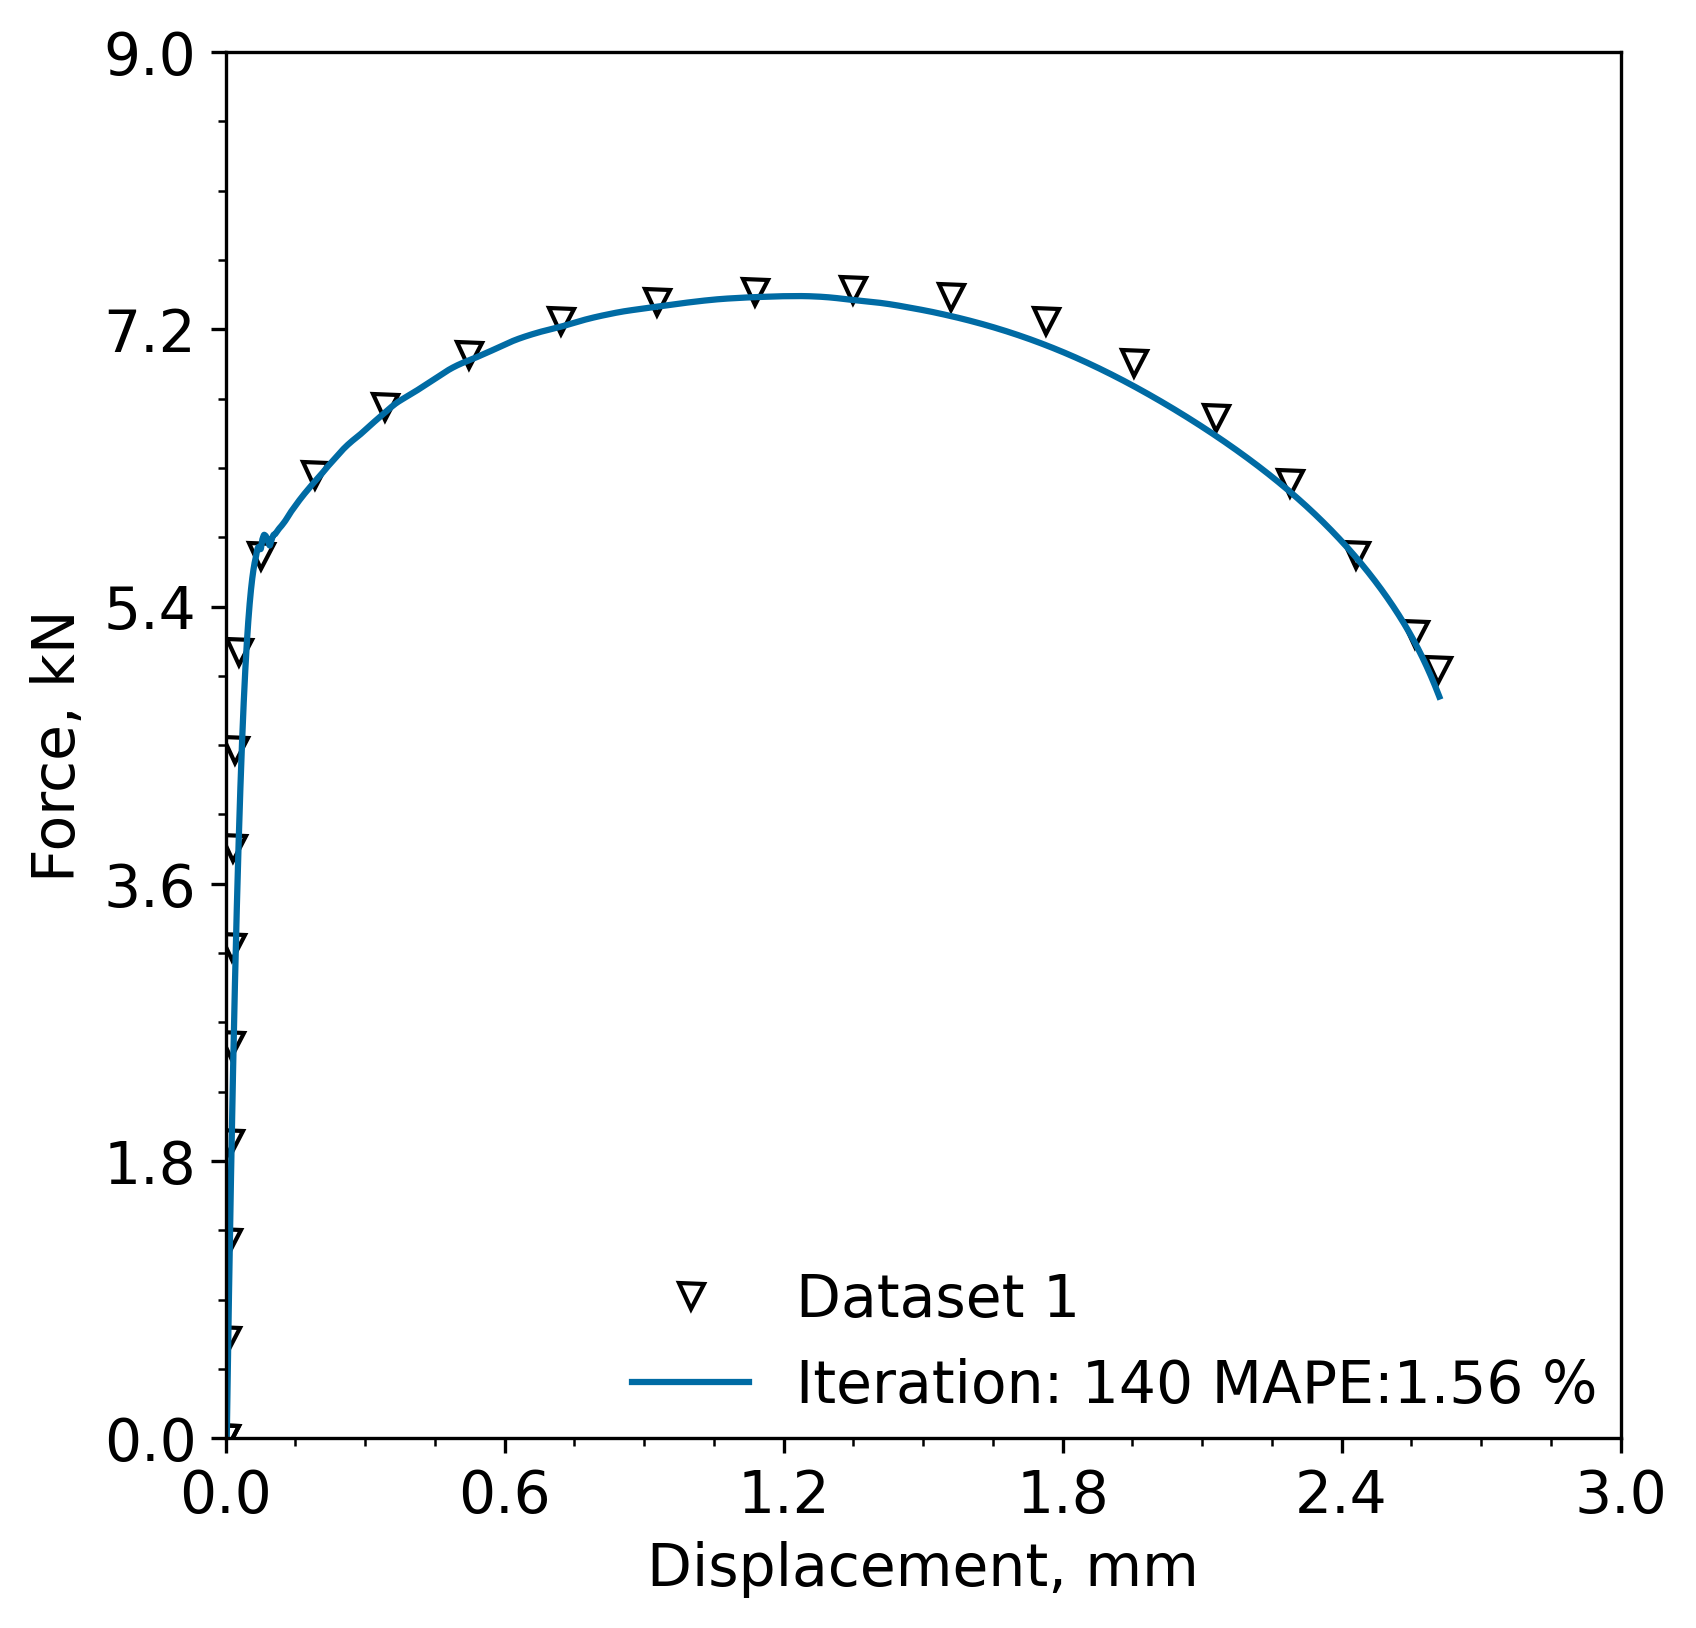
\includegraphics[width=\textwidth, height=0.45\textheight, keepaspectratio]{P91_20_2_FASTEST_ITERATION}
			\subcaption{Dataset 1}
			\label{fig:dataset1}
		\end{minipage}
	\hspace{0.2cm}
		\begin{minipage}[b]{0.5\linewidth}
			\centering
			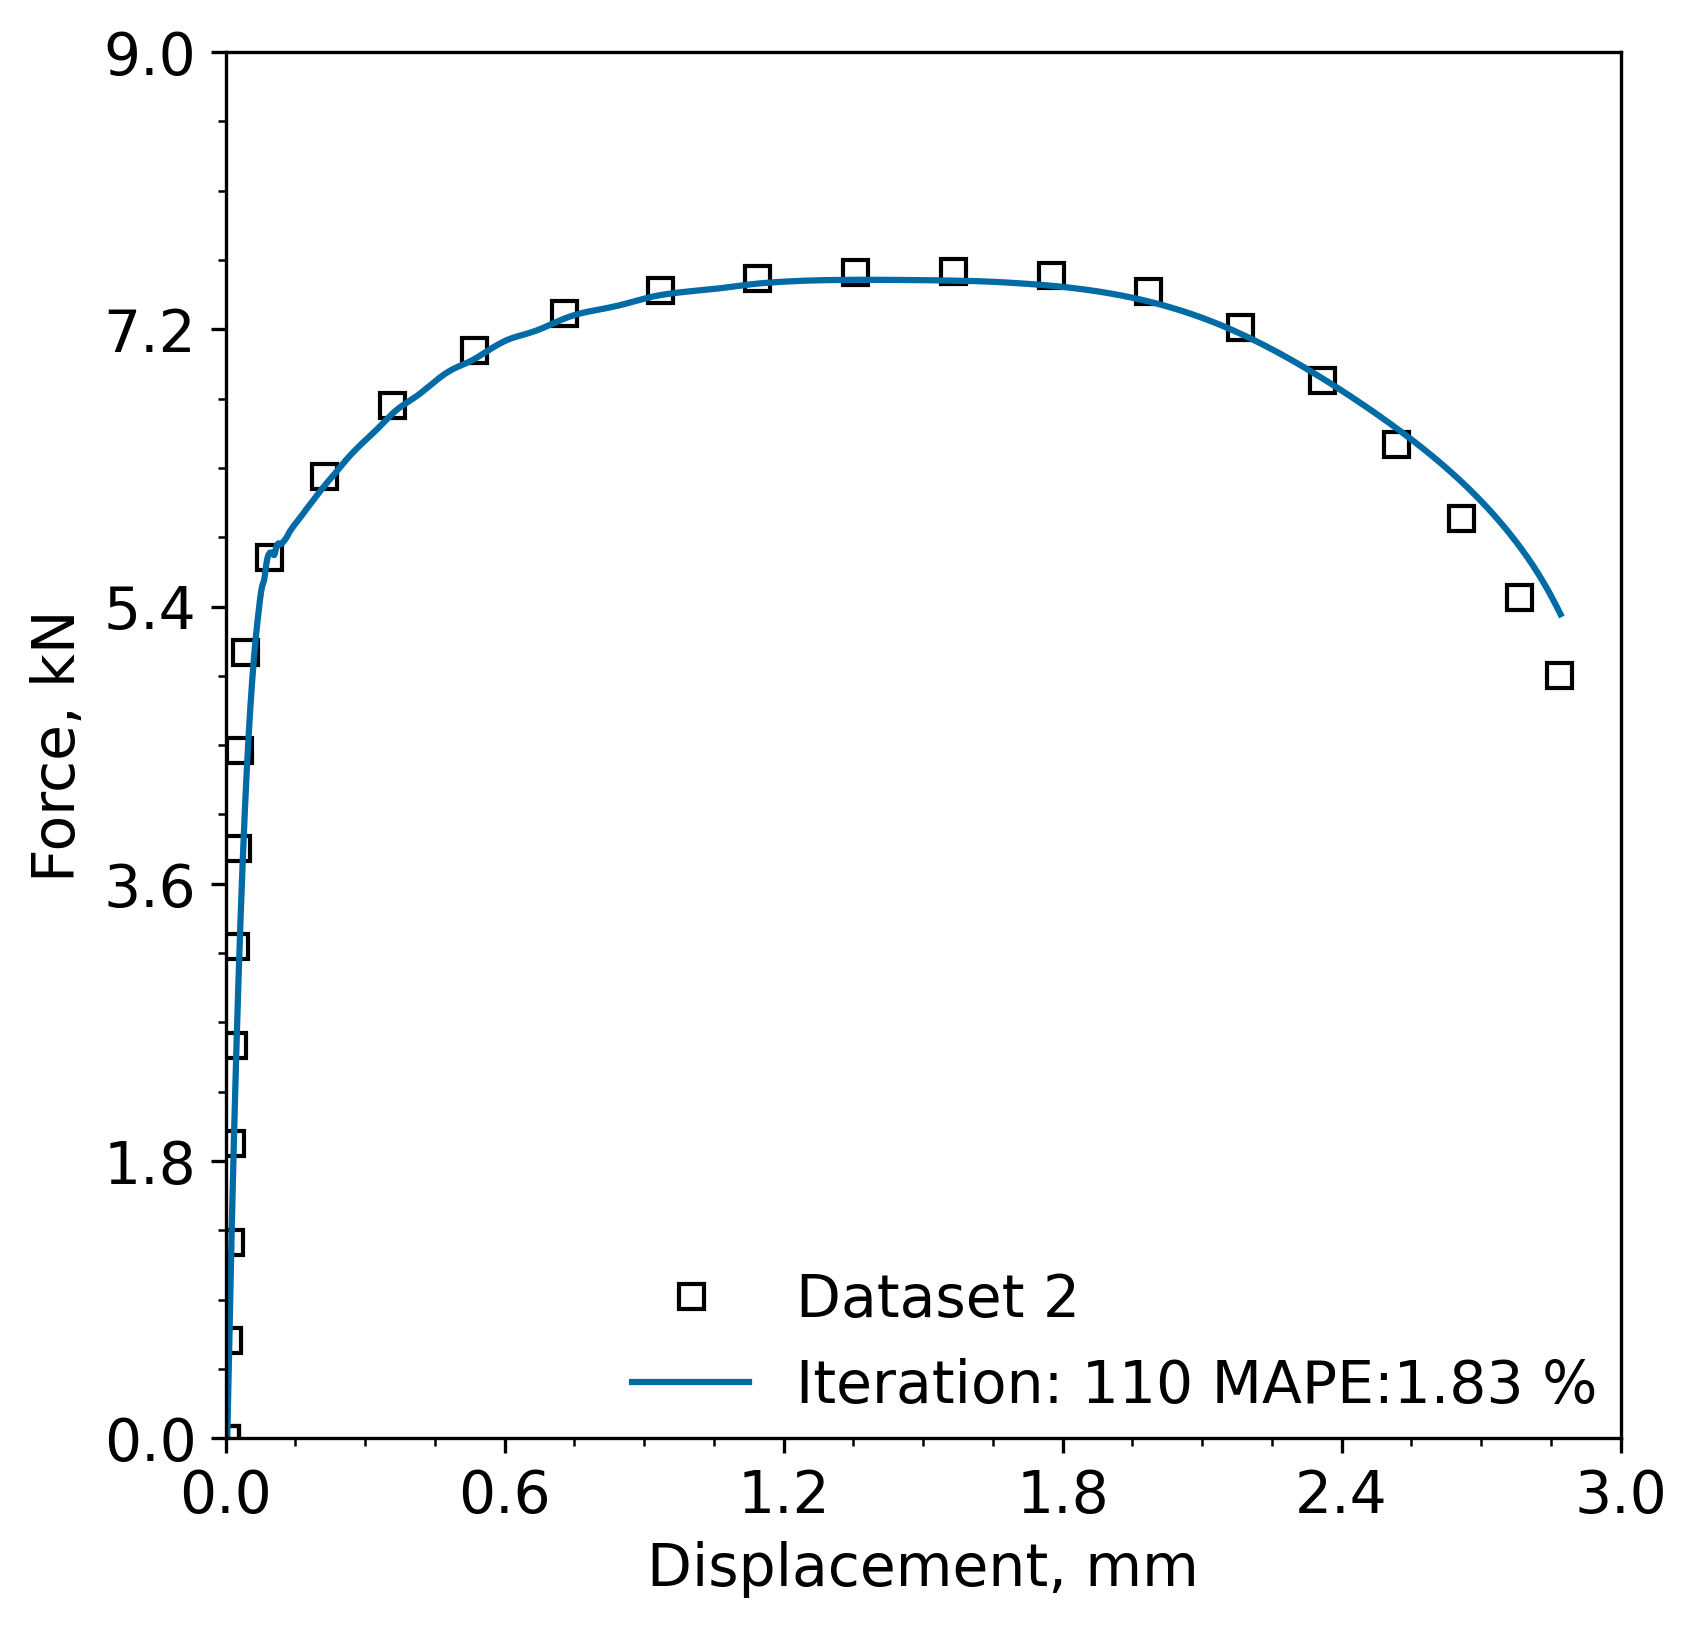
\includegraphics[width=\textwidth, height=0.45\textheight, keepaspectratio]{P91_20_1_FASTEST_ITERATION}
			\subcaption{Dataset 2}
			\label{fig:dataset2}
		\end{minipage}%%
	\vspace{0.2cm}
		\begin{minipage}[b]{\linewidth}
			\centering
			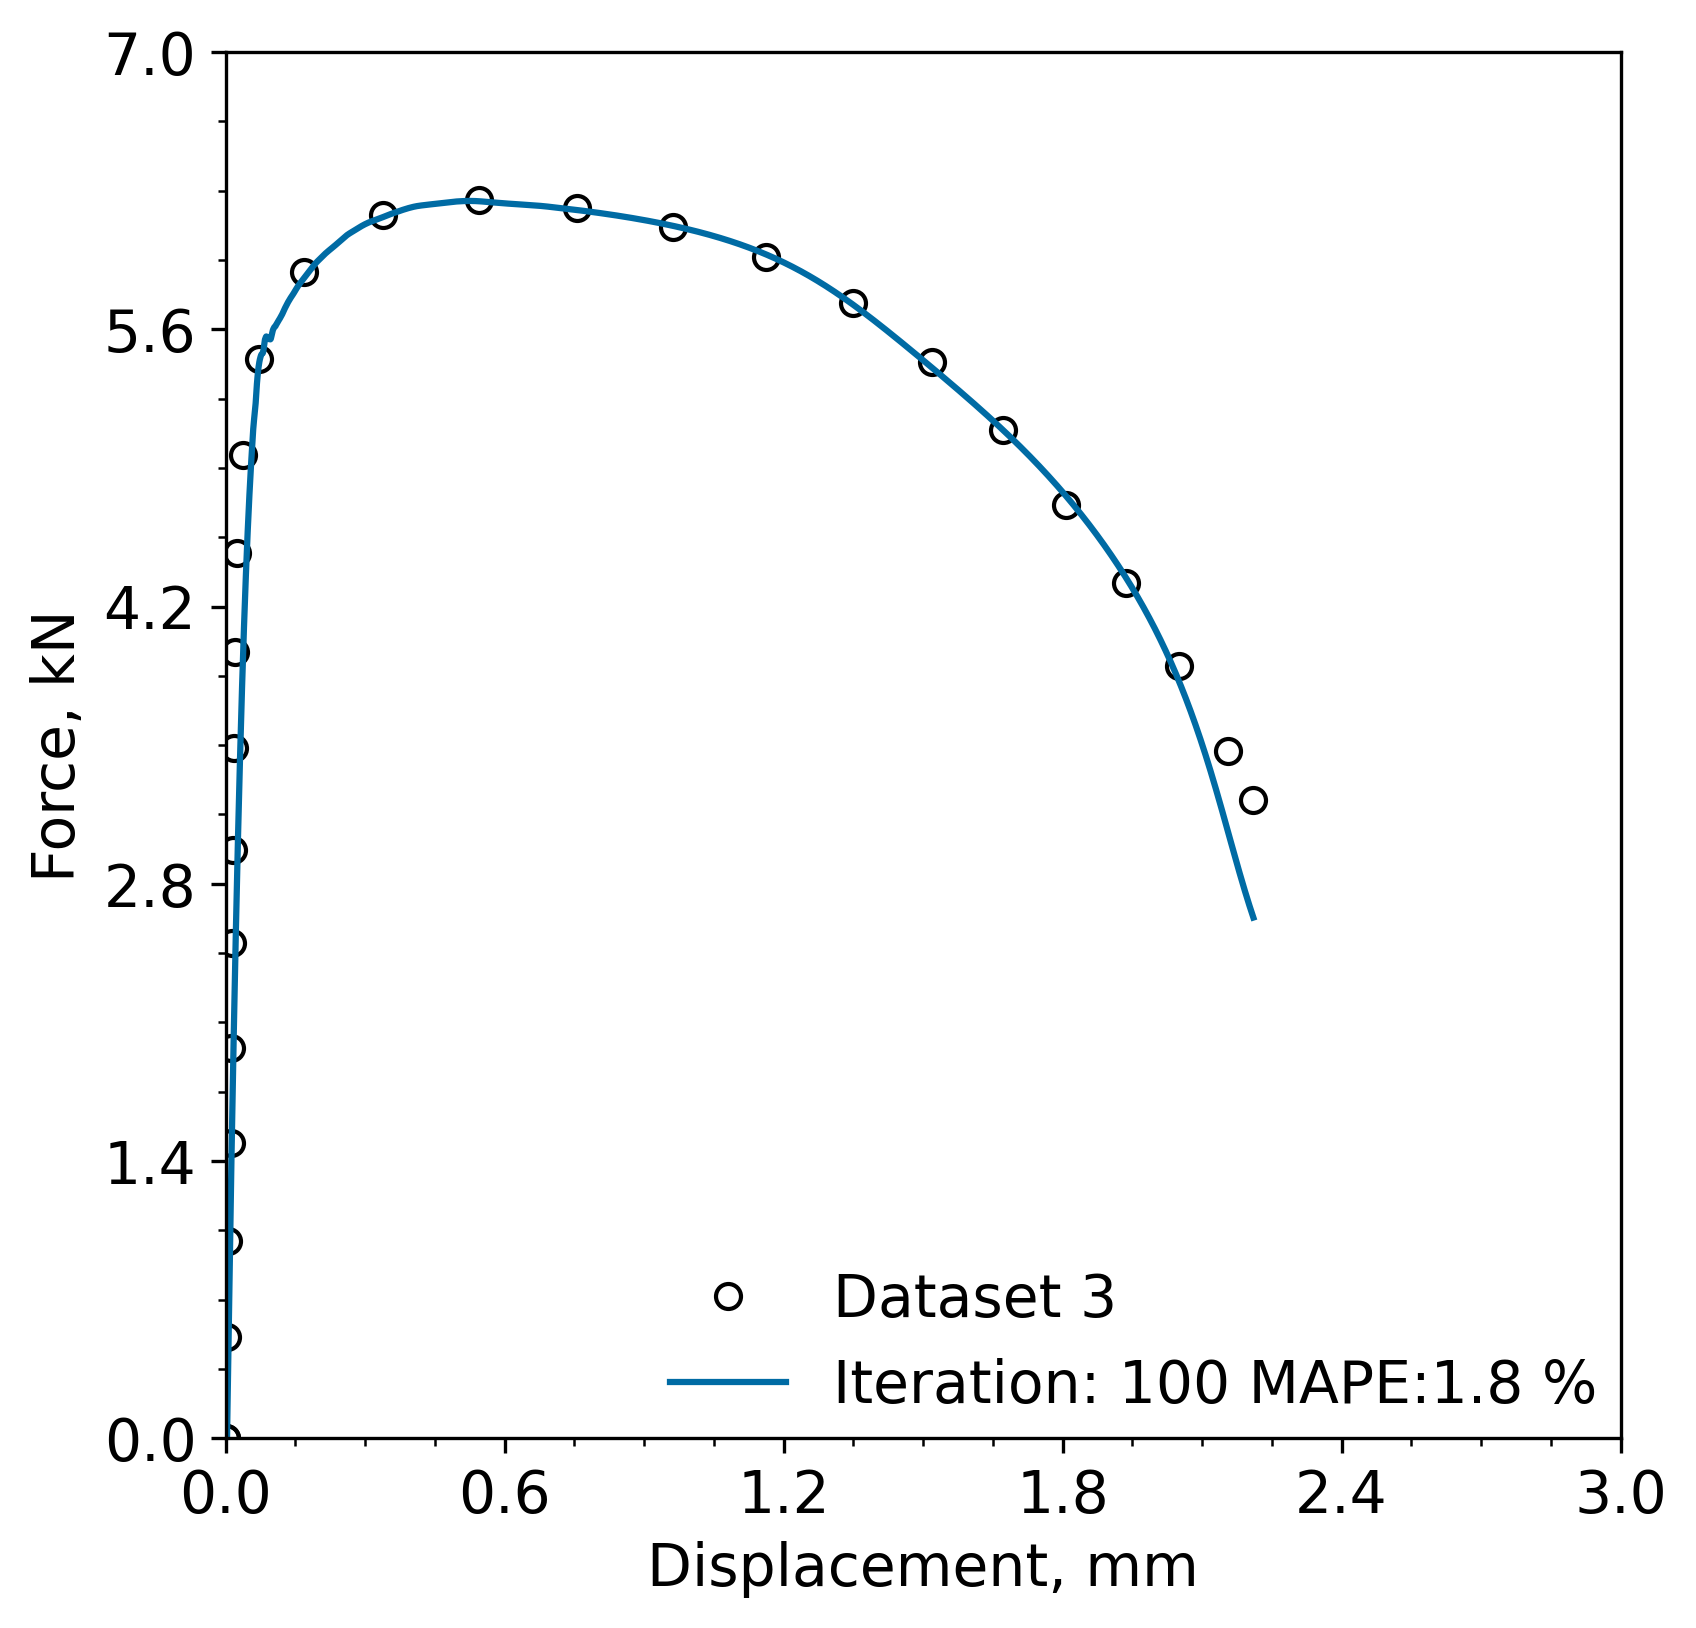
\includegraphics[width=0.5\textwidth, height=0.45\textheight, keepaspectratio]{P91_500_FASTEST_ITERATION}
			\subcaption{Dataset 3}
			\label{fig:dataset3}
		\end{minipage}~\caption{Comparison of experimental test data to simulated output for Dataset 1~(\ref{fig:dataset1}), Dataset 2~(\ref{fig:dataset2}), and Dataset 3~(\ref{fig:dataset3}). Parameter values are shown in Table~\ref{tab:bo_parameter_values}.}
	\label{fig:bo_result}
	\end{figure}


	\begin{table}[!htbp]
\centering
\caption{Bayesian optimisation framework parameter values for each of the three datasets analysed. }
\label{tab:bo_parameter_values}
\begin{tabular}{lccc}
\toprule
\textbf{Parameter} & \textbf{Dataset 1} & \textbf{Dataset 2} & \textbf{Dataset 3} \\
\midrule
$N_O$ & \multicolumn{3}{c}{500}\\
$N_R$ & \multicolumn{3}{c}{50,000}\\
%\multirow{2}{*}{\parbox{1.8cm}{Optimisation samples}} & \multicolumn{3}{c}{500}\\
%\\
%\multirow{2}{*}{\parbox{1.8cm}{Random samples}} & \multicolumn{3}{c}{50,000}\\
%\\
\midrule
%\textbf{$q_1$} &    1.3324 &    1.1684 &    1.1820 \\
%\textbf{$q_2$} &    0.9952 &    0.9667 &    0.9699 \\
%\textbf{$q_3$} &    2.2949 &    1.4071 &    2.0007 \\
%\textbf{$\epsilon_N$} &    0.2900 &    0.3467 &    0.3720 \\
%\textbf{$s_N$} &    0.1671 &    0.1856 &    0.1214 \\
%\textbf{$f_N$} &    0.0387 &    0.0848 &    0.0471 \\
%\textbf{$f_0$} &    1.374 \times 10^{-3} &    1.344 \times 10^{-3} &    1.310 \times 10^{ -3} \\
%\textbf{$m$} &  534.13 &  725.39 &  421.41 \\
%{MAPE} &    1.56 &    1.83 &    1.80 \\
%{Iteration number} &  140 &  110 &  100 \\
%% 4 SIGNIF FIGURES
\textbf{$q_1$} &    1.332 &    1.168 &    1.182 \\
\textbf{$q_2$} &    9.952\times10^{-1} &    9.667\times10^{-1} &    9.699\times10^{-1} \\
\textbf{$q_3$} &    2.295 &    1.407 &    2.001 \\
\textbf{$\epsilon_N$} &    2.900\times10^{-1} &    3.467\times10^{-1} &    3.720\times10^{-1} \\
\textbf{$s_N$} &    1.671\times10^{-1} &    1.856\times10^{-1} &    1.214\times10^{-1} \\
\textbf{$f_N$} &    3.869\times10^{-2} &    8.481\times10^{-2} &    4.706\times10^{-2} \\
\textbf{$f_0$} &    1.370 \times 10^{-3} &    1.340 \times 10^{-3} &    1.310 \times 10^{ -3} \\
\textbf{$m$} &  534.1 &  725.4 &  421.4 \\
{MAPE} &    1.563 &    1.827 &    1.799 \\
{$N_j$} &  140 &  110 &  100 \\
\bottomrule
\end{tabular}
\end{table}


	The tests for Dataset 1 and 2 have been carried out under nominally identical conditions, while the test for Dataset 3 has been carried out at a different temperature on the same material.

	The statistical nature of material's testing, often termed material scatter, has been widely acknowledged in the field of material science~\cite{OCONNOR2022}, so it is not unexpected that Dataset 1 and 2 differ and provide different calibrations to the GTN model.
	Indeed machine learning methods such as the ones employed here may be a useful tool to identify the reasons behind such experimental scatter.
	However, the limited data available in the current study are not sufficient, as such a study would require many repeat tests.

	It is interesting to note that parameter $m$, the slope of the extrapolated true stress-true strain curve was found to differ significantly between Datasets 1 and 2 (534~MPa and 725~MPa, respectively), although the load-displacement curves in Figure~\ref{fig:exp_test_results} are quite similar and almost identical below maximum load.
	It is also interesting to note that the parameter $f_0$, initial void volume fraction, is very similar for all three datasets (0.137\%, 0.134\%, 0.131\% for Dataset 1, 2 and 3, respectively).
	Generally the initial void volume fraction is not expected to vary significantly from specimen to specimen for a given material, which is consistent with what is observed here.
	However, parameters $\varepsilon_N$, $S_N$ and $f_N$, which control void nucleation, are also expected to be constant for a given material (at a given temperature), so the values for Dataset 1 and 2 would be expected to be similar.
	However, as seen in Table~\ref{tab:bo_parameter_values} there are significant differences, e.g.\ $f_N = 0.0387$ and $0.0848$ for Dataset 1 and 2, respectively.

	In terms of the fitting parameters ($q_1$, $q_2$ and $q_3$) it is common practice to fix $q_3 = q_1^2$~\cite{ABBASI2011,ROUSSELIER2019, YAN2021}, based on assumptions in the original model ~\cite{TVERGAARD1981a}.
	In this work, $q_3$ was not constrained and, as shown in Table~\ref{tab:bo_parameter_values}, Dataset 2 $q_3\approx q_1^2$, but the relationship does not hold for the other two datasets.
	Again, for definitive statement in relation to the significance of parameter values, a much larger data set would be needed, which is not the purpose of the current analysis.

	%%%%%%%%%%%%%%%%%
	\subsection{Effect of varying BO hyperparameters}
	\label{h:unique}

	To assess the effect of hyperparameter selection on the model parameters, four BO analyses were preformed on Dataset 1.
	For each analysis the acquisition function, $\alpha_{UCB}$ (see Section~\ref{h:acquisition_function}), hyperparameter values $N_R$ and $N_0$ were varied, as shown in Table~\ref{tab:hyper_parameter_values}.
	The load-displacement curves for the four cases are shown in Figure~\ref{fig:unique}.
	Excellent agreement with experimental data is achieved for the four hyperparameter choices.

	\begin{figure}[!htbp]
		\centering
		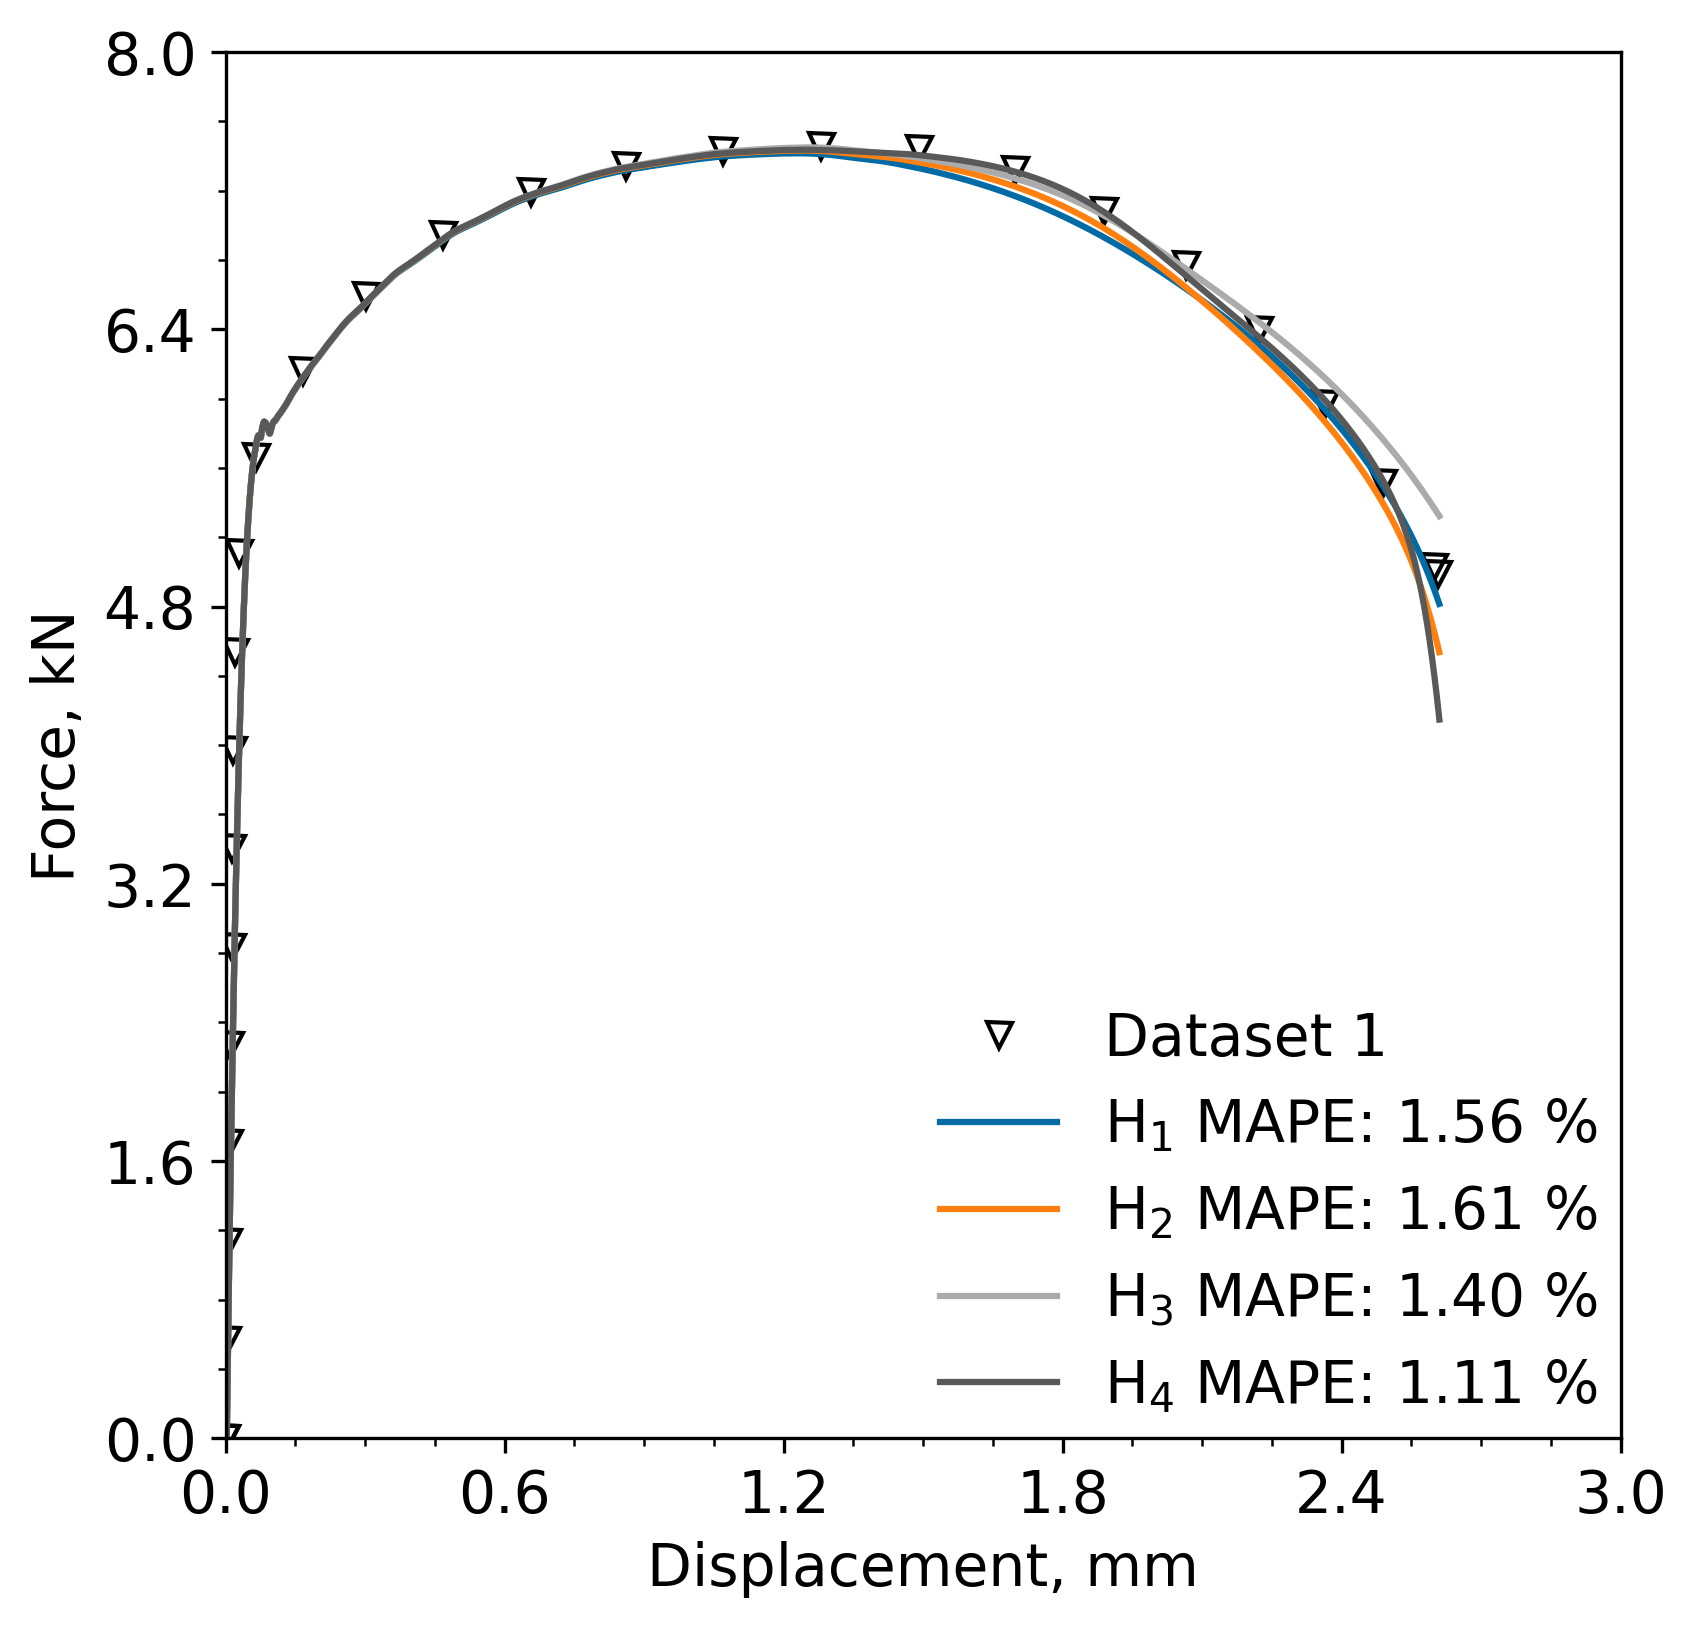
\includegraphics[width=\linewidth, height=0.4\textheight, keepaspectratio]{HYPERPARAMETERS}
		\caption{Plot of force versus displacement showing experimental data and simulated output for various hyperparameters.}
		\label{fig:unique}
	\end{figure}

	\begin{table}[!htbp]
\centering
\caption{Bayesian optimisation framework parameter values for dataset 1. The effect of hyperparameter settings on GTN parameter values. }
\label{tab:hyper_parameter_values}
\begin{tabular}{lcccc}
\toprule
\textbf{Parameter} & \textbf{$H_1$} & \textbf{$H_2$} & \textbf{$H_3$} & \textbf{$H_4$}\\
\midrule
$N_O$ & 500 & 100 & 500 & 100\\
$N_R$ & 50,000 & 50,000 & 10,000 & 10,000\\
%\multirow{2}{*}{\parbox{1.8cm}{Optimisation samples}} & \multirow{2}{*}{500} & \multirow{2}{*}{100} & \multirow{2}{*}{500} & \multirow{2}{*}{100}\\
%\\
%\multirow{2}{*}{\parbox{1.8cm}{Random samples}} & \multirow{2}{*}{50,000} & \multirow{2}{*}{50,000} & \multirow{2}{*}{10,000} & \multirow{2}{*}{10,000}\\
%\\
\midrule
%\textbf{$q_1$} & 1.3324 & 1.1775 & 1.2910 & 1.1578 \\
%\textbf{$q_2$} & 0.9952 & 1.0214 & 0.9547 & 1.0365 \\
%\textbf{$q_3$} & 2.2949 & 1.3443 & 2.2535 & 1.0702 \\
%\textbf{$\epsilon_N$} & 0.2900 & 0.3598 & 0.3517 & 0.3331 \\
%\textbf{$s_N$} & 0.1671 & 0.1580 & 0.1001 & 0.1234 \\
%\textbf{$f_N$} & 0.0387 & 0.0577 & 0.0309 & 0.0759 \\
%\textbf{$f_0$} & 1.374\times10^{-3} & 1.431\times10^{-3} & 1.412\times10^{-3} & 1.308\times10^{-3} \\
%\textbf{$m$}   & 534.13 & 542.79 & 514.54 & 621.85 \\
%{MAPE}         & 1.56 & 1.61 & 1.40 & 1.11 \\
%{Iteration number} & 140 & 133 & 46 & 130 \\
%% SIGNIFICANT FIGURES 4
\textbf{$q_1$} & 1.332 & 1.178 & 1.291 & 1.158 \\
%\textbf{$q_2$} & 0.9952 & 1.021 & 0.9547 & 1.037 \\
\textbf{$q_2$} & 9.952\times10^{-1} & 1.021 & 9.547\times10^{-1} & 1.037 \\
\textbf{$q_3$} & 2.295 & 1.344 & 2.254 & 1.070 \\
\textbf{$\epsilon_N$} & 2.900\times10^{-2} & 3.598\times10^{-1} & 3.519\times10^{-1} & 3.331\times10^{-1} \\
\textbf{$s_N$} & 1.671\times10^{-1} & 1.580\times10^{-1} & 1.001\times10^{-1} & 1.234\times10^{-1} \\
\textbf{$f_N$} & 3.869\times10^{-2} & 5.769\times10^{-2} & 3.086\times10^{-2} & 7.594\times10^{-2} \\
\textbf{$f_0$} & 1.370\times10^{-3} & 1.431\times10^{-3} & 1.412\times10^{-3} & 1.309\times10^{-3} \\
\textbf{$m$}   & 534.1 & 542.8 & 514.5 & 621.9 \\
{MAPE}         & 1.563 & 1.614 & 1.398 & 1.105 \\
{$N_j$} & 140 & 133 & 46 & 130 \\
\bottomrule
\end{tabular}
\end{table}


	 It may be noted from Table~\ref{tab:hyper_parameter_values} that all the model parameters depend on the hyperparameter selection.
	Given that excellent agreement was achieved for all four analyses this implies that the problem does not have a unique solution.
	That is to say that multiple combinations of the eight model parameters provide good agreement to the experimental data.

	The issue of non-uniqueness in GTN model parameter values has been highlighted by~\cite{KIRAN2014}.
	One method of uniquely identifying GTN parameters is to examine a second or even third test specimen geometry.
	As the GTN model, Equation~\ref{eq:gtn_yield}, is not specimen specific the model parameters should be applicable to any geometry.
	The proposed framework, can be extended to include multiple specimen types, by, for example, obtaining a range of potential GTN model parameters from one specimen type, carrying out a second BO analysis on the second specimen type within this range, and continuing with other specimen types until a unique set of parameters is achieved.
	\clearpage
	%%%%%%%%%%%%%%%%%%%%%%%%%%%
	\section{Conclusions}
	\label{h:conclusions}

	\begin{itemize}
		\item A Bayesian optimisation framework successfully determined an array of eight material parameter values that, when applied to a ductile damage model simulation, produced an accurate representation of experimental tensile data with a mean average percentage error (MAPE) of less than 2\%.
		\item The framework is fully autonomous requiring minimal user interaction with the combined machine learning-finite element tool typically provides calibration values in less than four hours.
		This compares favourably with typical time spent on trial-and-error calibration for this model.
		\item The ductile model parameter values are found to be non-unique and it is shown that by changing the hyperparameters of the acquistion function, different combinations of ductile damage parameters are obtained.
		\item Future work will consider how the BO framework can be adapted to obtain unique model parameters and how the approach can be applied to larger datasets and multiple specimen types.
	\end{itemize}

	%%%%%%%%%%%%%%%%%%%%%%%%%%%
	\section{Ackowledgements}
	\label{h:acknowledgements}

	This work was funded by the European Union through the Marie Sk{\l}owodska-Curie Actions grant number 101028291.
	We acknowledge William Brennan, a University of Limerick undergraduate student, for his contributions to this research.
	We gratefully acknowledge helpful conversations with Dr Meghana Kshiragar and Ms Gauri Vaidya from the University of Limerick's Lero Centre.
	We also acknowledge members of the University of Limerick, Mathematics Applications Consortium for Science and Industry (MACSI) group for their insightful and supportive comments surrounding this research.

	%%%%%%%%%%%%%%%%%%%%%%%%%%%
	\section{Supplementary information}
	\label{h:supplementary}

	A preprint of this research is available~\cite{OCONNOR2023}.
	Additional supplementary information such as data files and code are available from zenodo~\url{https://doi.org/10.5281/zenodo.7686217}.


%% If you have bibdatabase file and want bibtex to generate the
%% bibitems, please use
%
\bibliography{BO_PAPER}
\bibliographystyle{elsarticle-num-names}
	\biboptions{sort&compress}

\end{document}

\endinput
%%
%% End of file `elsarticle-template-num-names.tex